\chapter{Anexos}\label{anexos}

%%%%%%%%%%%%%%%%%%%%%%%%%%%%%%%%%%%%%%%%%%%%%%%%%%%%%%%%%%%%%%%%%%%%%%%%%%%%%%%%%%%%%%%%%%%%%%%%%%%%%%%%%%%%%%%%%%%%
\section{Resultados de los entrenamientos}\label{anexo-resultados-entrenamientos}

En esta sección se completan los resultados mostrados en el apartado \ref{analisis_entrenamientos} en relación a los resultados que devuelven las diferentes combinaciones de entrenamientos.

%%%%%%%%%%%%%%%%%%%%%%%%%%%%%%%%%%%%%%%%%%%%%%%%%%%%%%%%%%%%%%%%%%%%%%%%%%%%%%%%%%%%%%%%%%%%%%%%%%%%%%%%%%%%%%%%%%%%
\subsection{Circuito simple, conjunto de acciones medio y un punto de percepción}

\begin{figure}[!ht]
    \centering 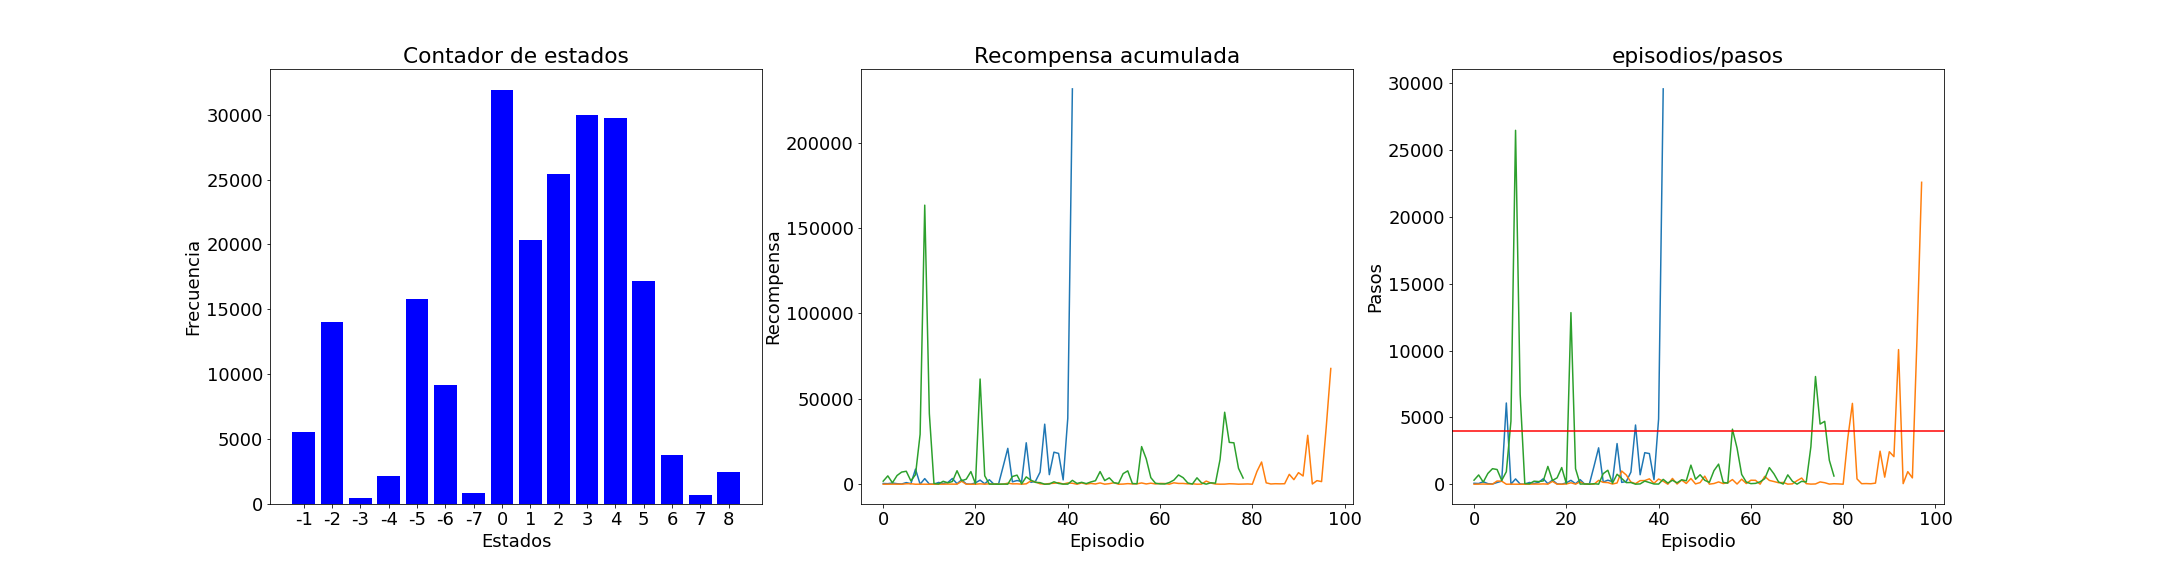
\includegraphics[width=1\columnwidth]{./figures/anexos/simple_circuit_medium_1.png}
    \caption{Gráfica de resultados del entrenamiento en el <<Circuito Simple>> con un conjunto de acciones medio y 1 punto de nivel de percepción.}
\end{figure}

\begin{table}[!ht]
\centering
\begin{tabular}{|
>{\columncolor[HTML]{EFEFEF}}l |c|c|c|}
\hline
\multicolumn{4}{|c|}{\cellcolor[HTML]{EFEFEF}\textbf{Tabla de entrenamiento en el Circuito Simple}}                                   \\ \hline
\textbf{Entrenamiento} & \cellcolor[HTML]{3685BB}\textbf{1} & \cellcolor[HTML]{FF8215}\textbf{2} & \cellcolor[HTML]{2CA02C}\textbf{3} \\ \hline
\textbf{Vuelta completada}         & Sí        & Sí        & Sí        \\ \hline
\textbf{Tiempo hasta completar}    & 05:19 min & 21:32 min & 10:33 min \\ \hline
\textbf{Épocas hasta completar}    & 7         & 82        & 8         \\ \hline
\textbf{Valor de $\epsilon$ final} & 0.81      & 0.76      & 0.79      \\ \hline
\textbf{Tamaño de la Tabla-Q}      & 53        & 55        & 33        \\ \hline
\textbf{Nº total de épocas}        & 42        & 98        & 79        \\ \hline
\end{tabular}
\caption{Resultados del entrenamiento en el <<Circuito Simple>> con un conjunto de acciones medio y 1 punto de nivel de percepción.}
\label{tab:simple_circuit-medium-1}
\end{table}


\newpage
%%%%%%%%%%%%%%%%%%%%%%%%%%%%%%%%%%%%%%%%%%%%%%%%%%%%%%%%%%%%%%%%%%%%%%%%%%%%%%%%%%%%%%%%%%%%%%%%%%%%%%%%%%%%%%%%%%%%
\subsection{Circuito simple, conjunto de acciones difícil y un punto de percepción}

\begin{figure}[h!]
    \centering 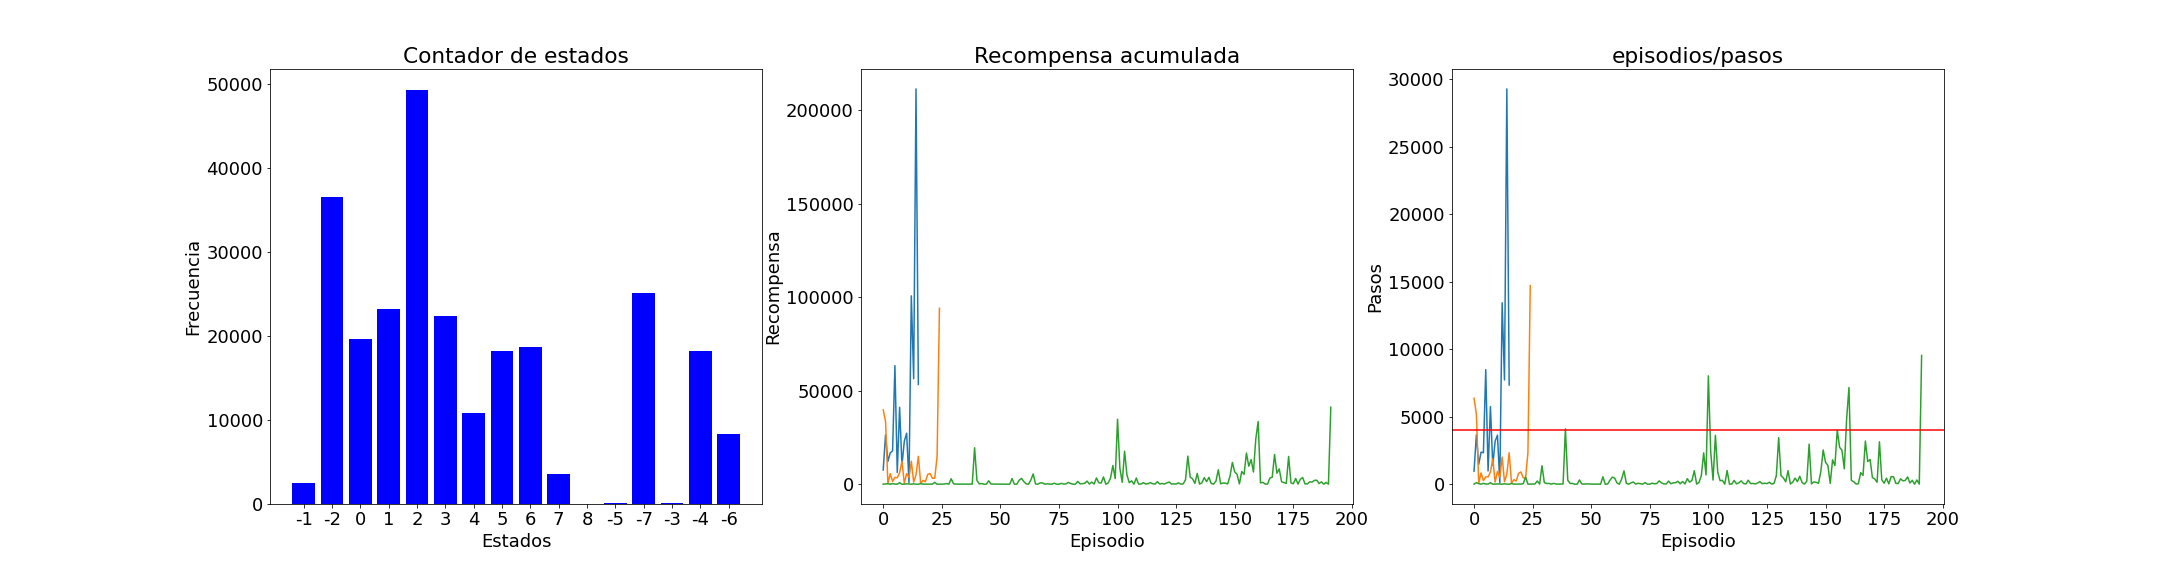
\includegraphics[width=1\columnwidth]{./figures/anexos/simple_circuit_hard_1.png}
    \caption{Gráfica de resultados del entrenamiento en el <<Circuito Simple>> con un conjunto de acciones difícil y 1 punto de nivel de percepción.}
\end{figure}

\begin{table}[h!]
\centering
\begin{tabular}{|
>{\columncolor[HTML]{EFEFEF}}l |c|c|c|}
\hline
\multicolumn{4}{|c|}{\cellcolor[HTML]{EFEFEF}\textbf{Tabla de entrenamiento en el Circuito Simple}}                                   \\ \hline
\textbf{Entrenamiento} & \cellcolor[HTML]{3685BB}\textbf{1} & \cellcolor[HTML]{FF8215}\textbf{2} & \cellcolor[HTML]{2CA02C}\textbf{3} \\ \hline
\textbf{Vuelta completada}         & Sí        & Sí        & Sí         \\ \hline
\textbf{Tiempo hasta completar}    & 16:28 min & 04:28 min & 08:07 min  \\ \hline
\textbf{Épocas hasta completar}    & 5         & 1         & 39         \\ \hline
\textbf{Valor de $\epsilon$ final} & 0.84      & 0.80      & 0.68       \\ \hline
\textbf{Tamaño de la Tabla-Q}      & 27        & 29        & 73         \\ \hline
\textbf{Nº total de épocas}        & 16        & 25        & 192        \\ \hline
\end{tabular}
\caption{Resultados del entrenamiento en el <<Circuito Simple>> con un conjunto de acciones difícil y 1 punto de nivel de percepción.}
\label{tab:simple_circuit-medium-1}
\end{table}


\newpage
%%%%%%%%%%%%%%%%%%%%%%%%%%%%%%%%%%%%%%%%%%%%%%%%%%%%%%%%%%%%%%%%%%%%%%%%%%%%%%%%%%%%%%%%%%%%%%%%%%%%%%%%%%%%%%%%%%%%
\subsection{Circuito simple, conjunto de acciones simple y dos puntos de percepción}

\begin{figure}[ht!]
    \centering 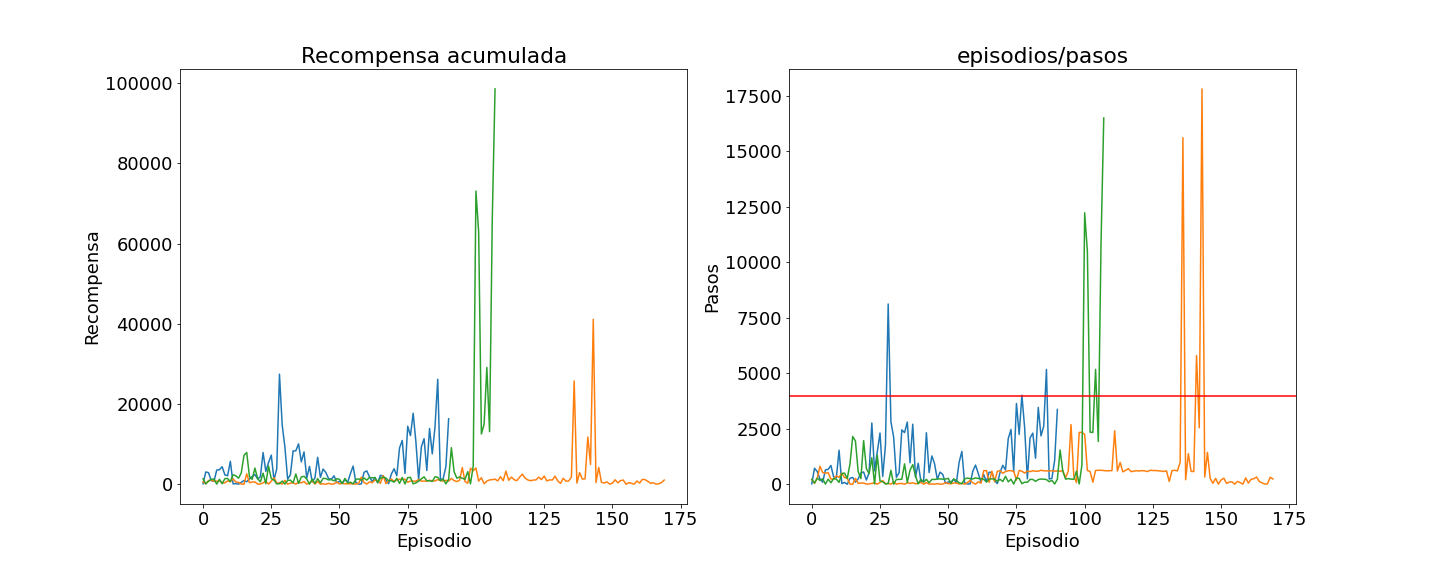
\includegraphics[width=1\columnwidth]{./figures/anexos/simple_circuit_simple_2.png}
    \caption{Gráfica de resultados del entrenamiento en el <<Circuito Simple>> con un conjunto de acciones simple y 2 puntos de nivel de percepción.}
\end{figure}

\begin{figure}[ht!]
    \centering 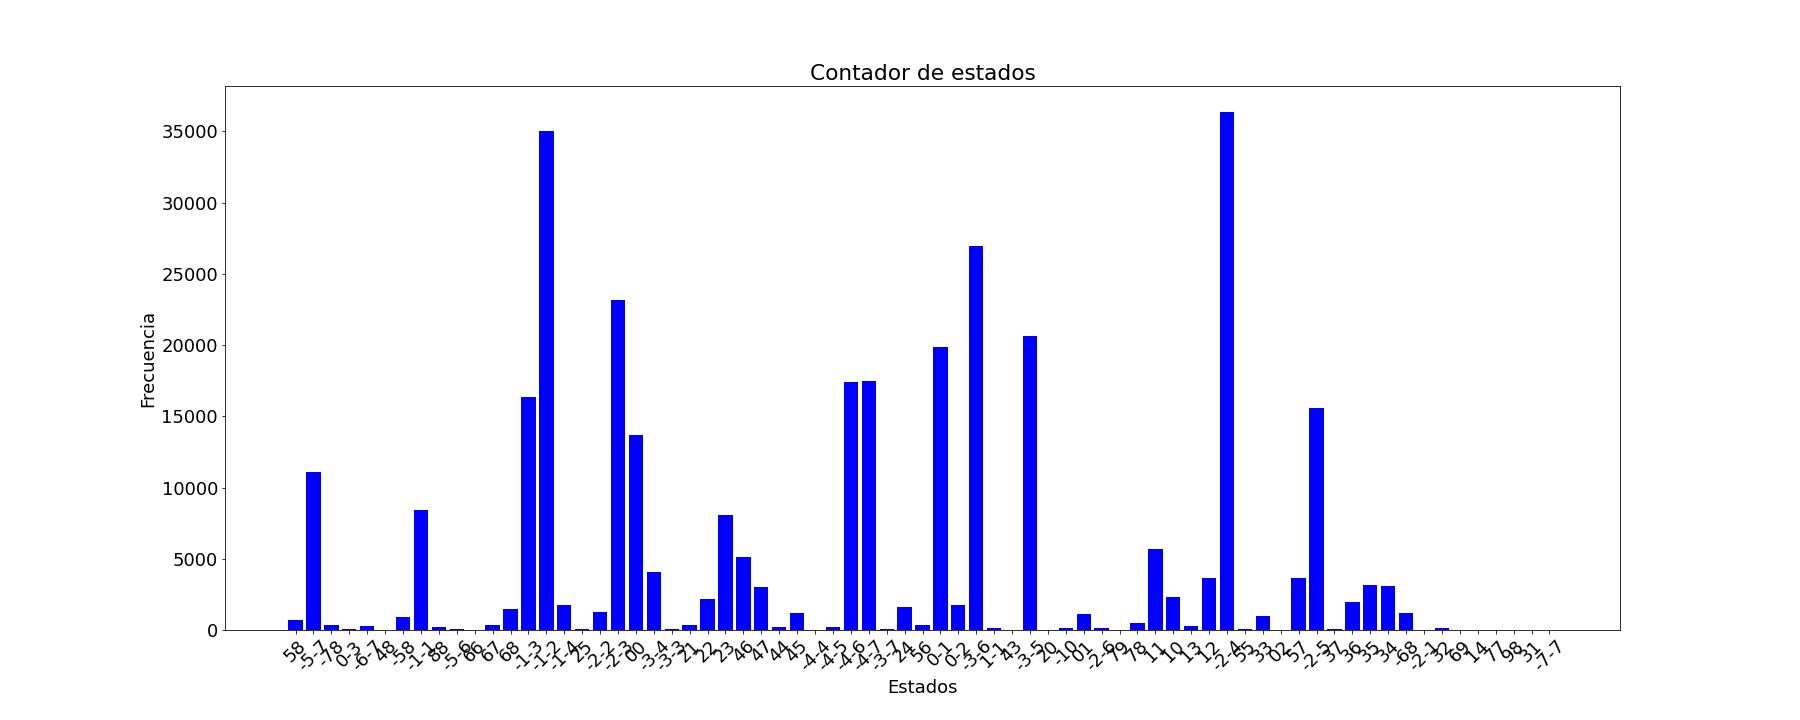
\includegraphics[width=1\columnwidth]{./figures/anexos/states_counter_simple_circuit_simple_2.png}
    \caption{Gráfica de resultados de la distribución de los estados.}
\end{figure}

\begin{table}[ht!]
\centering
\begin{tabular}{|
>{\columncolor[HTML]{EFEFEF}}l |c|c|c|}
\hline
\multicolumn{4}{|c|}{\cellcolor[HTML]{EFEFEF}\textbf{Tabla de entrenamiento en el Circuito Simple}}                                   \\ \hline
\textbf{Entrenamiento} & \cellcolor[HTML]{3685BB}\textbf{1} & \cellcolor[HTML]{FF8215}\textbf{2} & \cellcolor[HTML]{2CA02C}\textbf{3} \\ \hline
\textbf{Vuelta completada}         & Sí        & Sí        & Sí        \\ \hline
\textbf{Tiempo hasta completar}    & 1:23:35 horas & 1:09:11 horas min & 41:55 min \\ \hline
\textbf{Épocas hasta completar}    & 77         & 136        & 100         \\ \hline
\textbf{Valor de $\epsilon$ final} & 0.79      & 0.73      & 0.76      \\ \hline
\textbf{Tamaño de la Tabla-Q}      & 106        & 126        & 93        \\ \hline
\textbf{Nº total de épocas}        & 91        & 170        & 108        \\ \hline
\end{tabular}
\caption{Resultados del entrenamiento en el <<Circuito Simple>> con un conjunto de acciones simple y 2 puntos de nivel de percepción.}
\label{tab:simple_circuit-medium-1}
\end{table}


\newpage
%%%%%%%%%%%%%%%%%%%%%%%%%%%%%%%%%%%%%%%%%%%%%%%%%%%%%%%%%%%%%%%%%%%%%%%%%%%%%%%%%%%%%%%%%%%%%%%%%%%%%%%%%%%%%%%%%%%%
\subsection{Circuito simple, conjunto de acciones medio y dos puntos de percepción}

\begin{figure}[!ht]
    \centering 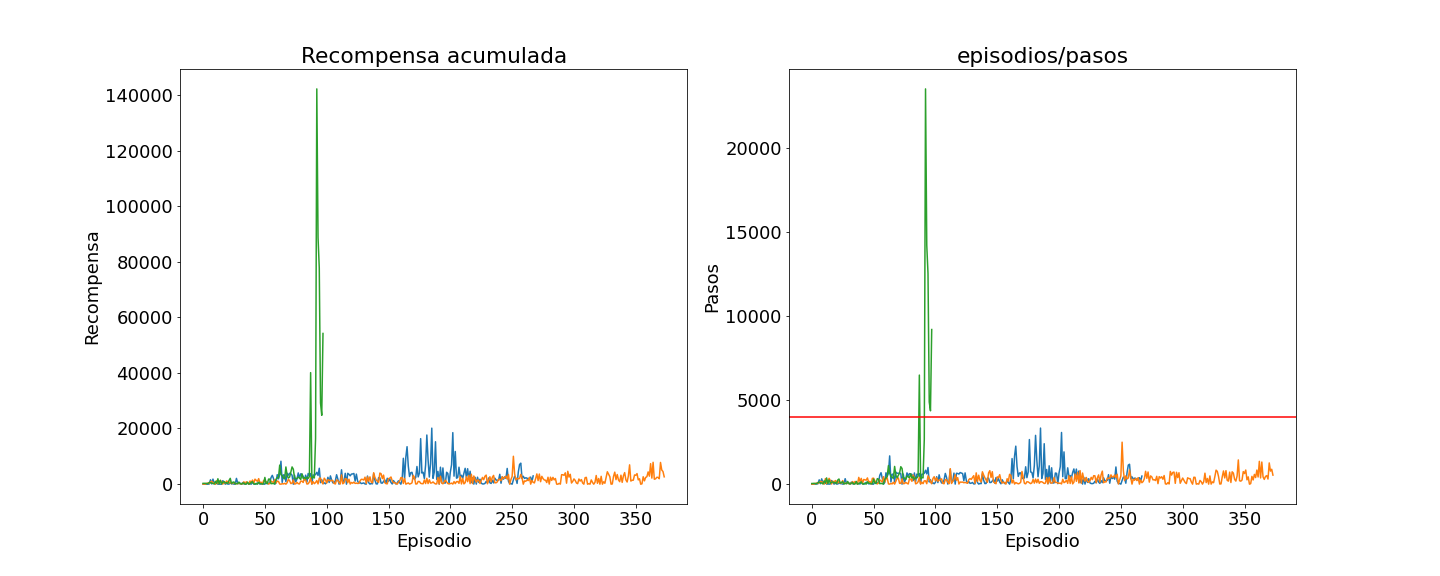
\includegraphics[width=1\columnwidth]{./figures/anexos/simple_circuit_medium_2.png}
    \caption{Gráfica de resultados del entrenamiento en el <<Circuito Simple>> con un conjunto de acciones medio y 2 puntos de nivel de percepción.}
\end{figure}

\begin{figure}[!ht]
    \centering 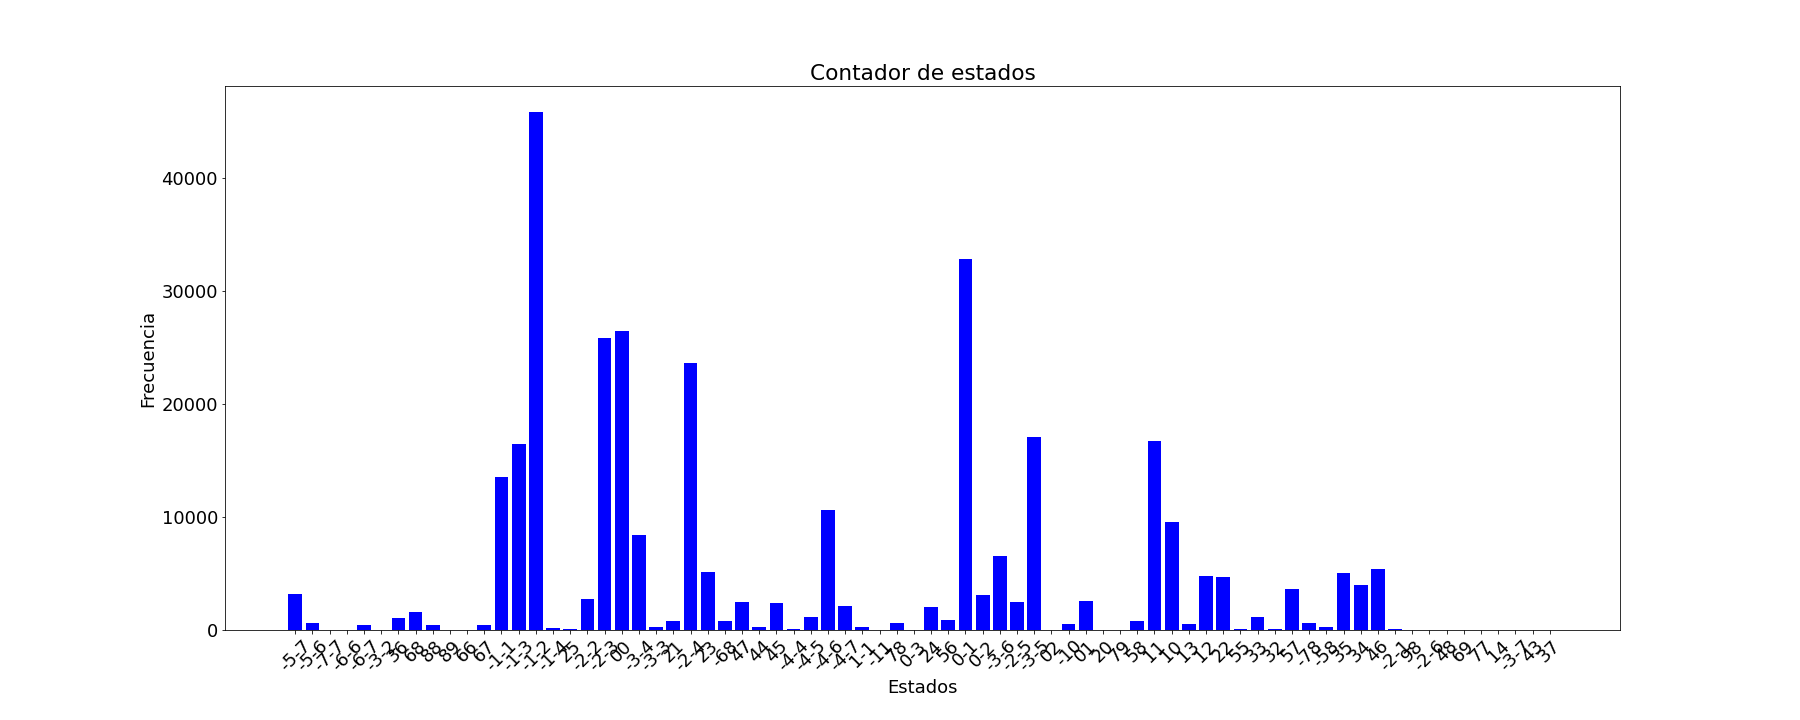
\includegraphics[width=1\columnwidth]{./figures/anexos/states_counter_simple_circuit_medium_2.png}
    \caption{Gráfica de resultados de la distribución de los estados.}
\end{figure}

\begin{table}[ht!]
\centering
\begin{tabular}{|
>{\columncolor[HTML]{EFEFEF}}l |c|c|c|}
\hline
\multicolumn{4}{|c|}{\cellcolor[HTML]{EFEFEF}\textbf{Tabla de entrenamiento en el Circuito Simple}}                                   \\ \hline
\textbf{Entrenamiento} & \cellcolor[HTML]{3685BB}\textbf{1} & \cellcolor[HTML]{FF8215}\textbf{2} & \cellcolor[HTML]{2CA02C}\textbf{3} \\ \hline
\textbf{Vuelta completada}         & No        & No          & Sí        \\ \hline
\textbf{Tiempo hasta completar}    & $\infty$  & $\infty$    & 26:55 min \\ \hline
\textbf{Épocas hasta completar}    & -         & -           & 87         \\ \hline
\textbf{Valor de $\epsilon$ final} & 0.65      & 0.58        & 0.67      \\ \hline
\textbf{Tamaño de la Tabla-Q}      & 163       & 168         & 115        \\ \hline
\textbf{Nº total de épocas}        & 268       & 374         & 97        \\ \hline
\end{tabular}
\caption{Resultados del entrenamiento en el <<Circuito Simple>> con un conjunto de acciones medio y 2 puntos de nivel de percepción.}
\label{tab:simple_circuit-medium-1}
\end{table}






















\newpage
%%%%%%%%%%%%%%%%%%%%%%%%%%%%%%%%%%%%%%%%%%%%%%%%%%%%%%%%%%%%%%%%%%%%%%%%%%%%%%%%%%%%%%%%%%%%%%%%%%%%%%%%%%%%%%%%%%%%
\subsection{Circuito simple, conjunto de acciones difícil y dos puntos de percepción}

\begin{figure}[!ht]
    \centering 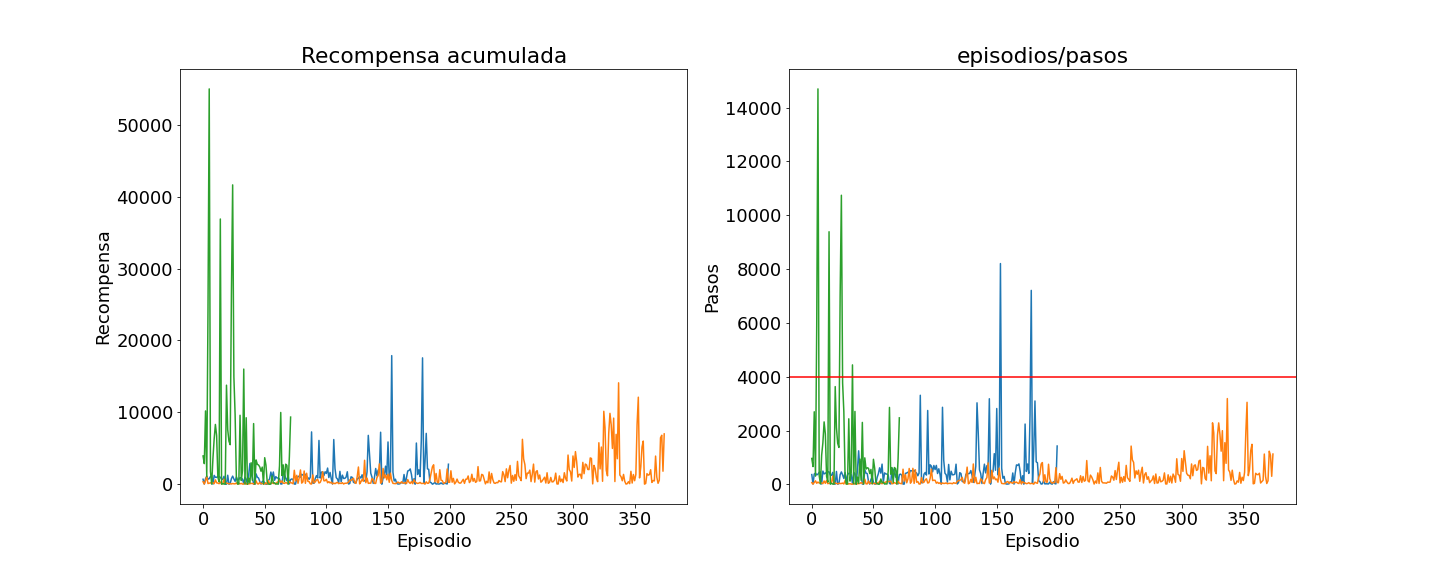
\includegraphics[width=1\columnwidth]{./figures/anexos/simple_circuit_hard_2.png}
    \caption{Gráfica de resultados del entrenamiento en el <<Circuito Simple>> con un conjunto de acciones difícil y 2 puntos de nivel de percepción.}
\end{figure}

\begin{figure}[!ht]
    \centering 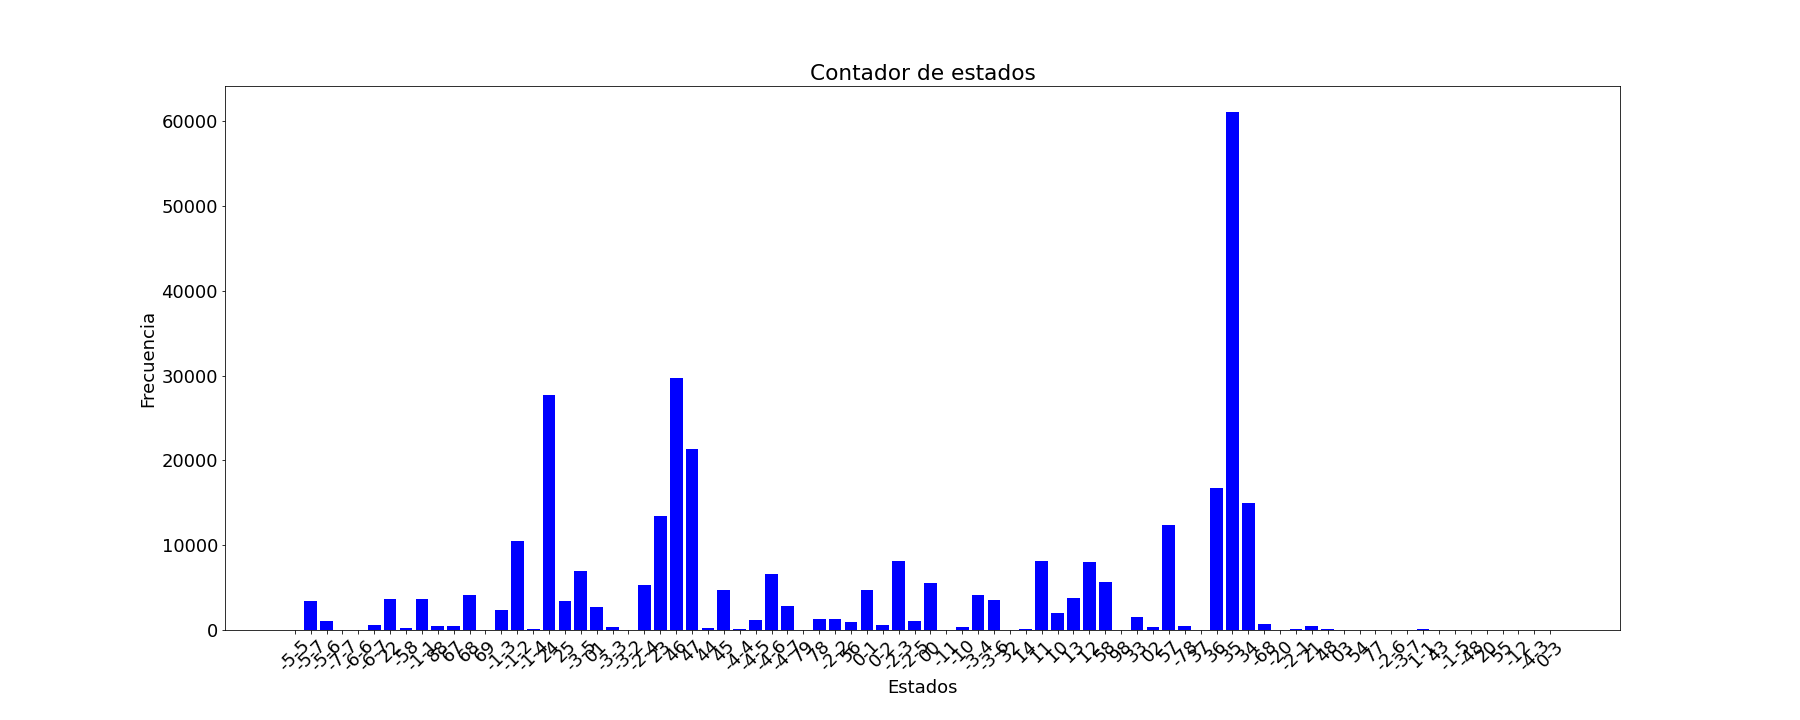
\includegraphics[width=1\columnwidth]{./figures/anexos/states_counter_simple_circuit_hard_2.png}
    \caption{Gráfica de resultados de la distribución de los estados.}
\end{figure}

\begin{table}[ht!]
\centering
\begin{tabular}{|
>{\columncolor[HTML]{EFEFEF}}l |c|c|c|}
\hline
\multicolumn{4}{|c|}{\cellcolor[HTML]{EFEFEF}\textbf{Tabla de entrenamiento en el Circuito Simple}}                                   \\ \hline
\textbf{Entrenamiento} & \cellcolor[HTML]{3685BB}\textbf{1} & \cellcolor[HTML]{FF8215}\textbf{2} & \cellcolor[HTML]{2CA02C}\textbf{3} \\ \hline
\textbf{Vuelta completada}         & Sí        & Sí          & Sí        \\ \hline
\textbf{Tiempo hasta completar}    & 1:25:03 horas  & 1:58:26 horas    & 09:30 min \\ \hline
\textbf{Épocas hasta completar}    & 153         & 375           & 4         \\ \hline
\textbf{Valor de $\epsilon$ final} & 0.70      & 0.56        & 0.80      \\ \hline
\textbf{Tamaño de la Tabla-Q}      & 184       & 214         & 123        \\ \hline
\textbf{Nº total de épocas}        & 200       & 375         & 72        \\ \hline
\end{tabular}
\caption{Resultados del entrenamiento en el <<Circuito Simple>> con un conjunto de acciones difícil y 2 puntos de nivel de percepción.}
\label{tab:simple_circuit-medium-1}
\end{table}


















\newpage
%%%%%%%%%%%%%%%%%%%%%%%%%%%%%%%%%%%%%%%%%%%%%%%%%%%%%%%%%%%%%%%%%%%%%%%%%%%%%%%%%%%%%%%%%%%%%%%%%%%%%%%%%%%%%%%%%%%%
\subsection{Circuito simple, conjunto de acciones simple y tres puntos de percepción}

El estado más frecuente es el  $(137)$ con un valor de $32382$ veces.

\begin{figure}[!ht]
    \centering 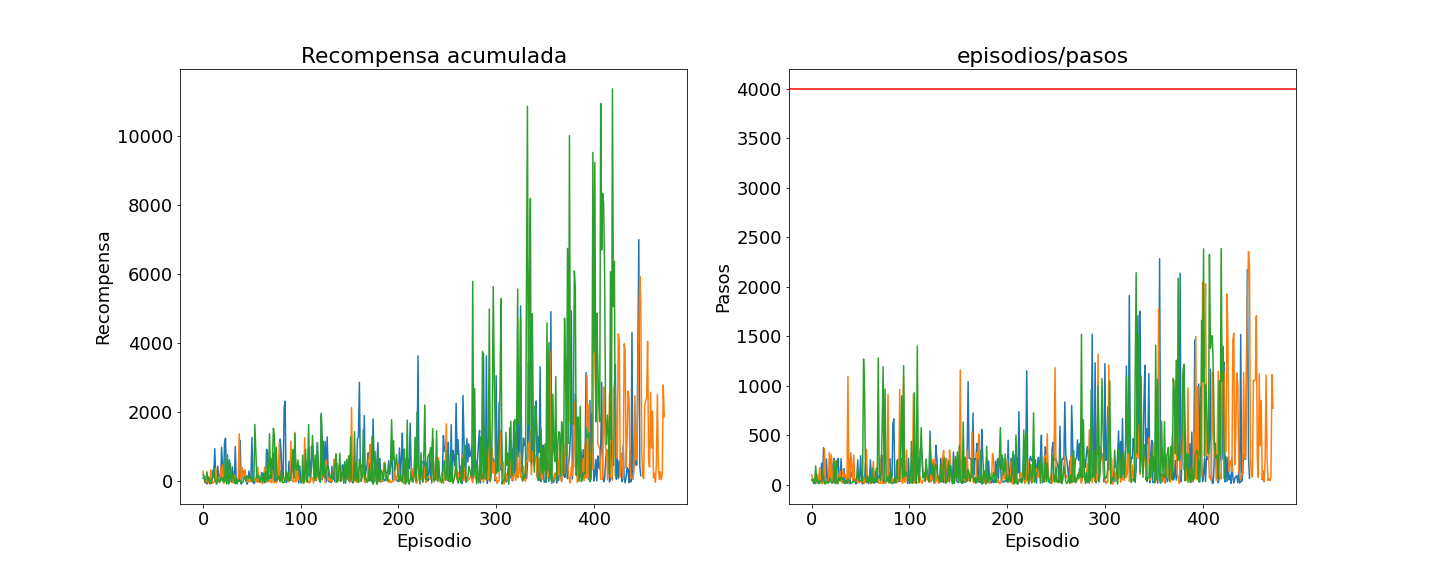
\includegraphics[width=1\columnwidth]{./figures/anexos/simple_circuit_simple_3.png}
    \caption{Gráfica de resultados del entrenamiento en el <<Circuito Simple>> con un conjunto de acciones simple y 3 puntos de nivel de percepción.}
\end{figure}

\begin{figure}[!ht]
    \centering 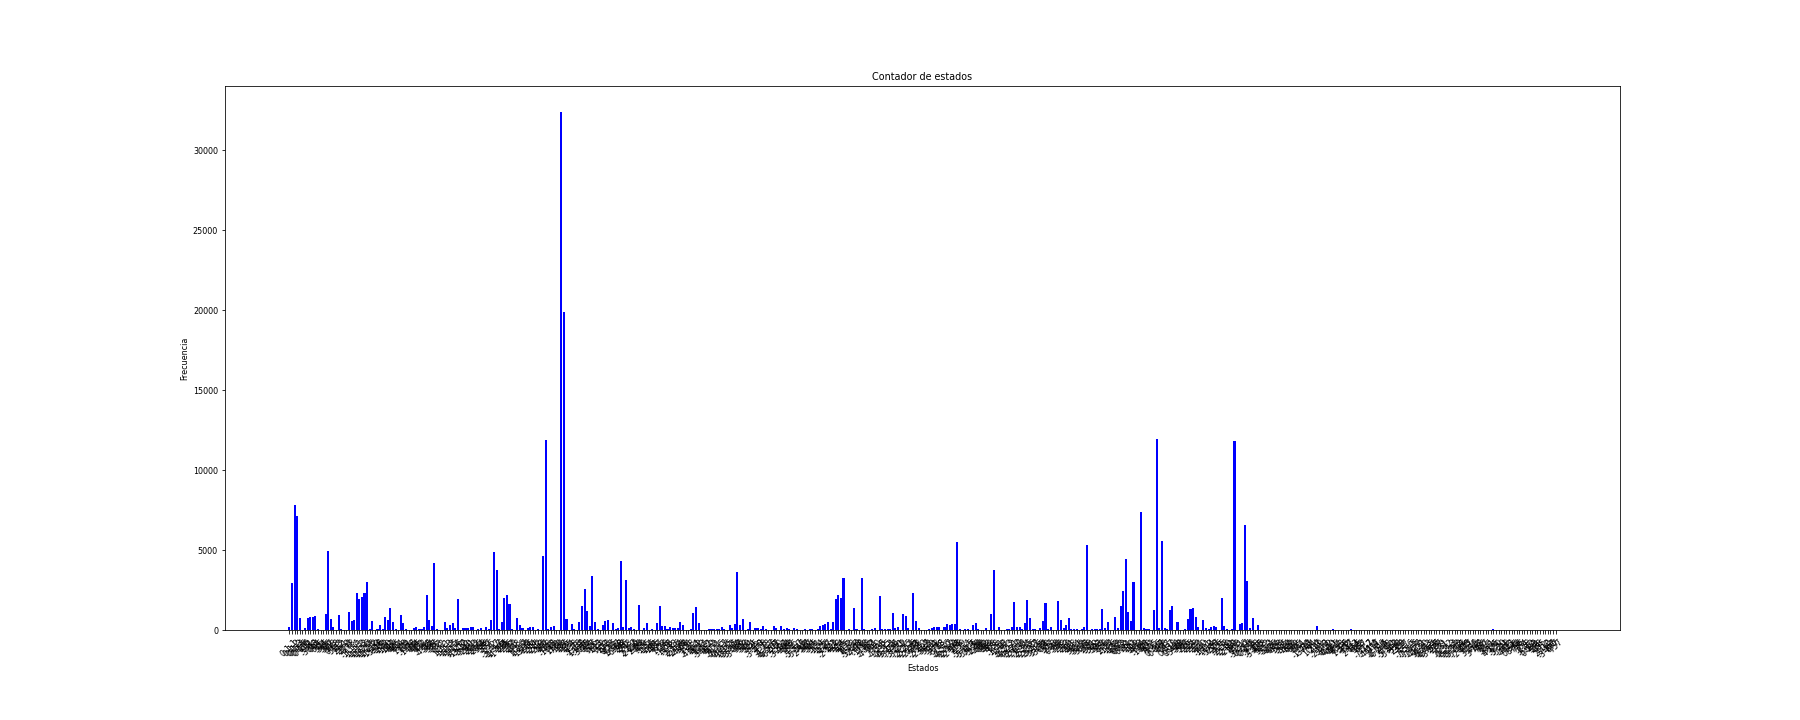
\includegraphics[width=1\columnwidth]{./figures/anexos/states_counter_simple_circuit_simple_3.png}
    \caption{Gráfica de resultados de la distribución de los estados.}
\end{figure}

\begin{table}[ht!]
\centering
\begin{tabular}{|
>{\columncolor[HTML]{EFEFEF}}l |c|c|c|}
\hline
\multicolumn{4}{|c|}{\cellcolor[HTML]{EFEFEF}\textbf{Tabla de entrenamiento en el Circuito Simple}}                                   \\ \hline
\textbf{Entrenamiento} & \cellcolor[HTML]{3685BB}\textbf{1} & \cellcolor[HTML]{FF8215}\textbf{2} & \cellcolor[HTML]{2CA02C}\textbf{3} \\ \hline
\textbf{Vuelta completada}         & No        & No          & No        \\ \hline
\textbf{Tiempo hasta completar}    & $\infty$  & $\infty$    & $\infty$ \\ \hline
\textbf{Épocas hasta completar}    & -         & -      & -         \\ \hline
\textbf{Valor de $\epsilon$ final} & 0.51      & 0.48        & 0.52      \\ \hline
\textbf{Tamaño de la Tabla-Q}      & 590       & 702         & 626        \\ \hline
\textbf{Nº total de épocas}        & 449       & 473         & 424        \\ \hline
\end{tabular}
\caption{Resultados del entrenamiento en el <<Circuito Simple>> con un conjunto de acciones simple y 3 puntos de nivel de percepción.}
\label{tab:simple_circuit-medium-1}
\end{table}


\newpage
%%%%%%%%%%%%%%%%%%%%%%%%%%%%%%%%%%%%%%%%%%%%%%%%%%%%%%%%%%%%%%%%%%%%%%%%%%%%%%%%%%%%%%%%%%%%%%%%%%%%%%%%%%%%%%%%%%%%
\subsection{Circuito simple, conjunto de acciones medio y tres puntos de percepción}

El estado más frecuente es el  $(1,3,7)$ con un valor de $10698$ veces.

\begin{figure}[!ht]
    \centering 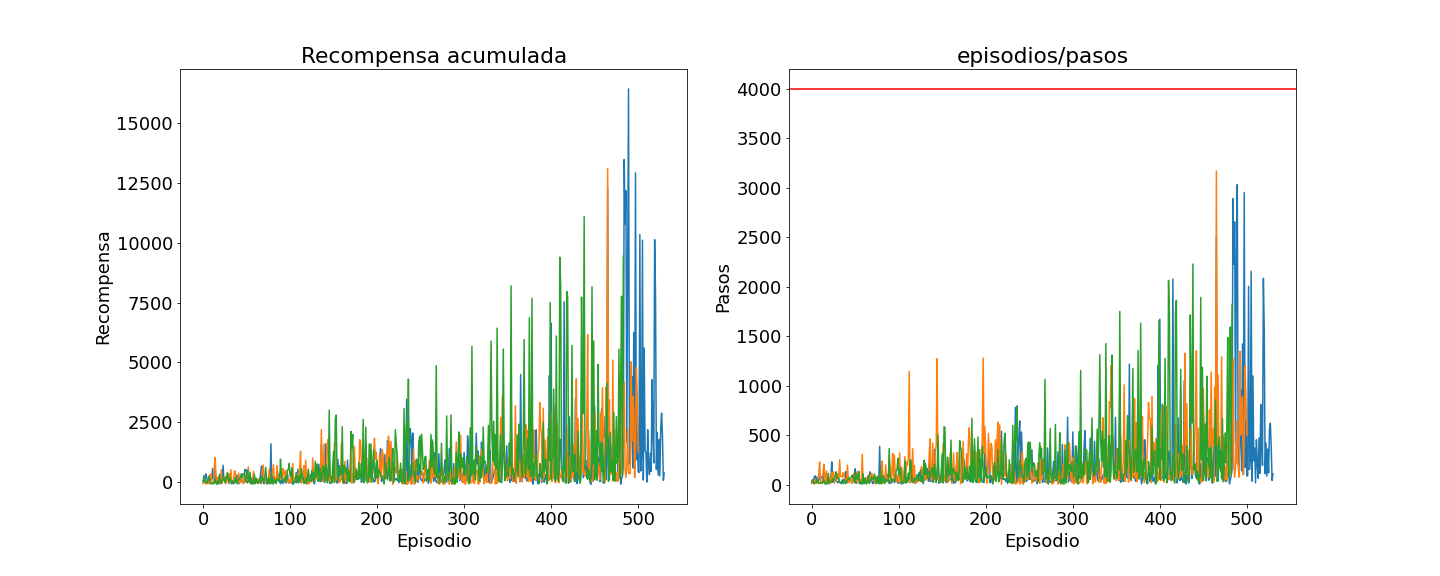
\includegraphics[width=1\columnwidth]{./figures/anexos/simple_circuit_medium_3.png}
    \caption{Gráfica de resultados del entrenamiento en el <<Circuito Simple>> con un conjunto de acciones medio y 3 puntos de nivel de percepción.}
\end{figure}

\begin{figure}[!ht]
    \centering 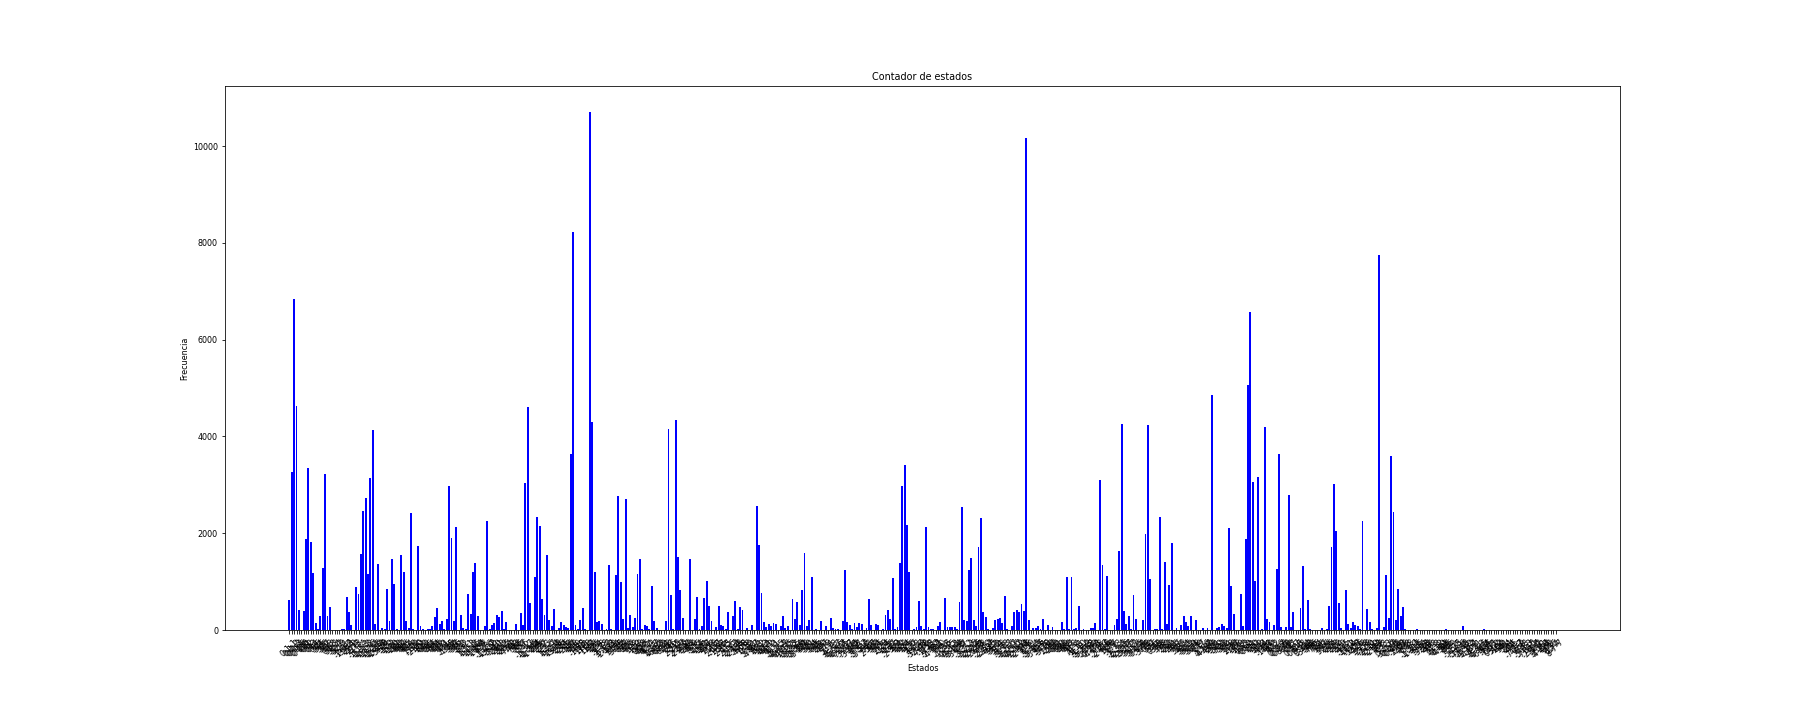
\includegraphics[width=1\columnwidth]{./figures/anexos/states_counter_simple_circuit_medium_3.png}
    \caption{Gráfica de resultados de la distribución de los estados.}
\end{figure}

\begin{table}[ht!]
\centering
\begin{tabular}{|
>{\columncolor[HTML]{EFEFEF}}l |c|c|c|}
\hline
\multicolumn{4}{|c|}{\cellcolor[HTML]{EFEFEF}\textbf{Tabla de entrenamiento en el Circuito Simple}}                                   \\ \hline
\textbf{Entrenamiento} & \cellcolor[HTML]{3685BB}\textbf{1} & \cellcolor[HTML]{FF8215}\textbf{2} & \cellcolor[HTML]{2CA02C}\textbf{3} \\ \hline
\textbf{Vuelta completada}         & No        & No          & No        \\ \hline
\textbf{Tiempo hasta completar}    & $\infty$  & $\infty$    & $\infty$ \\ \hline
\textbf{Épocas hasta completar}    & -         & -      & -              \\ \hline
\textbf{Valor de $\epsilon$ final} & 0.45      & 0.48        & 0.48      \\ \hline
\textbf{Tamaño de la Tabla-Q}      & 857       & 745         & 792        \\ \hline
\textbf{Nº total de épocas}        & 531       & 501         & 484        \\ \hline
\end{tabular}
\caption{Resultados del entrenamiento en el <<Circuito Simple>> con un conjunto de acciones medio y 3 puntos de nivel de percepción.}
\label{tab:simple_circuit-medium-1}
\end{table}


\newpage
%%%%%%%%%%%%%%%%%%%%%%%%%%%%%%%%%%%%%%%%%%%%%%%%%%%%%%%%%%%%%%%%%%%%%%%%%%%%%%%%%%%%%%%%%%%%%%%%%%%%%%%%%%%%%%%%%%%%
\subsection{Circuito simple, conjunto de acciones difícil y tres puntos de percepción}

El estado más frecuente es el  $(0, -2, -6)$ con un valor de $12814$ veces.

\begin{figure}[!ht]
    \centering 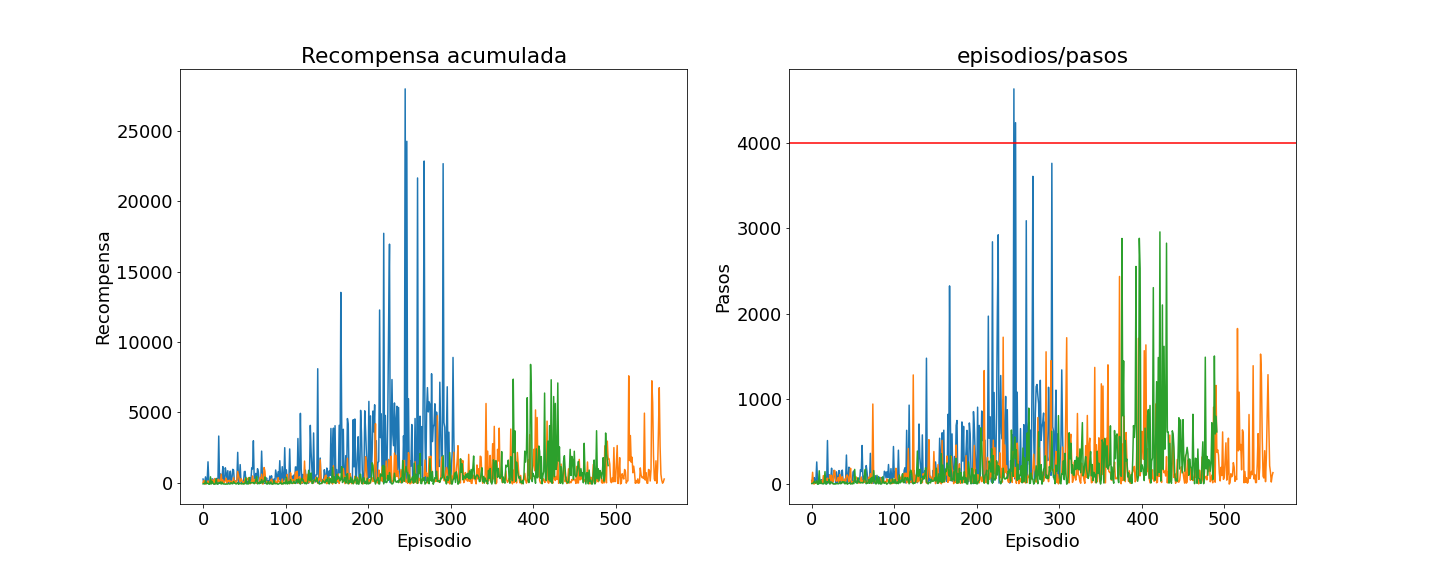
\includegraphics[width=1\columnwidth]{./figures/anexos/simple_circuit_hard_3.png}
    \caption{Gráfica de resultados del entrenamiento en el <<Circuito Simple>> con un conjunto de acciones difícil y 3 puntos de nivel de percepción.}
\end{figure}

\begin{figure}[!ht]
    \centering 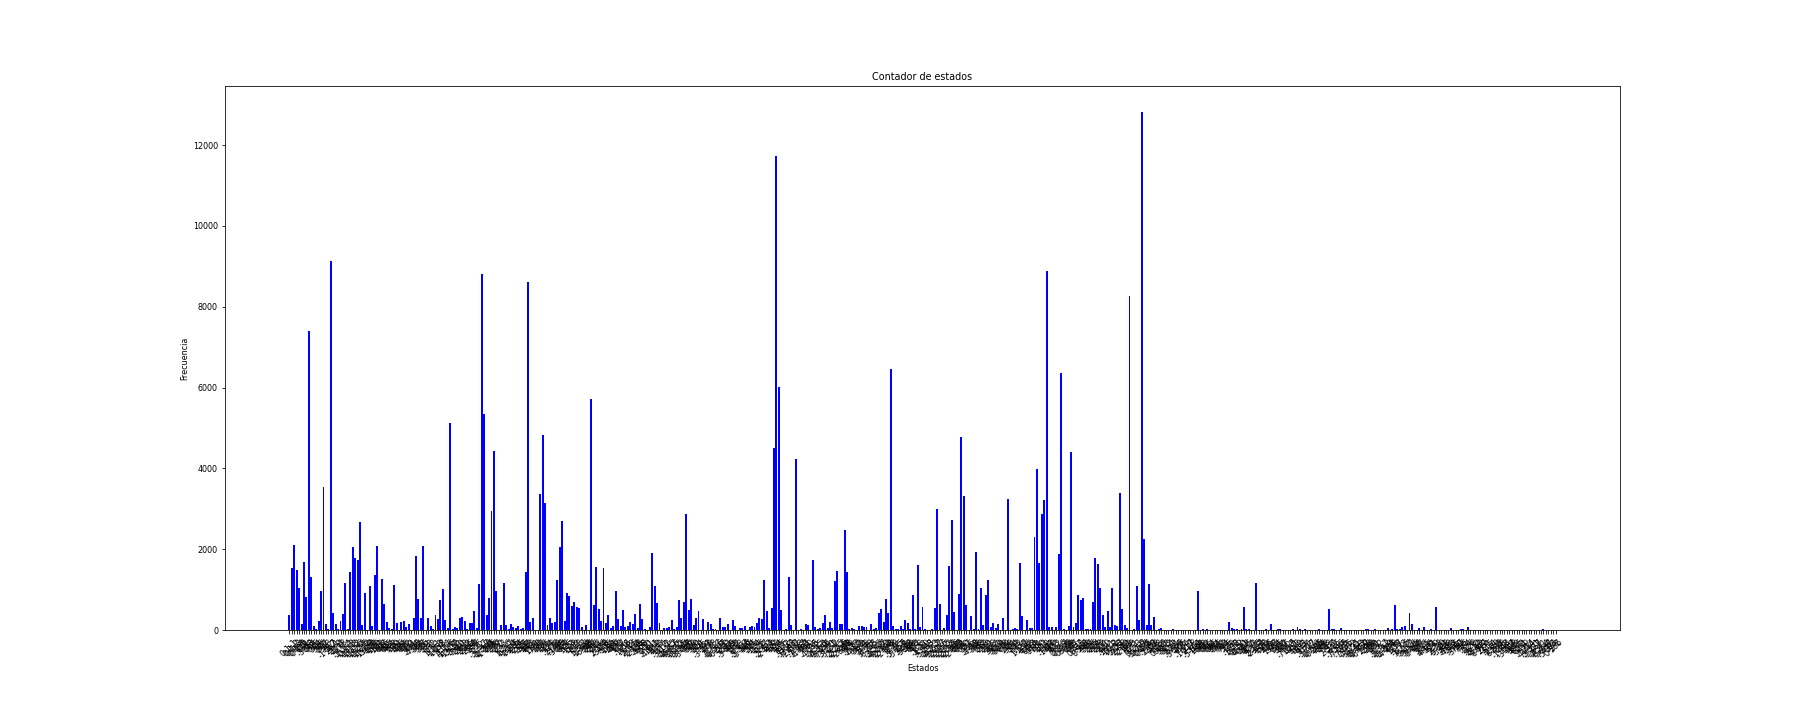
\includegraphics[width=1\columnwidth]{./figures/anexos/states_counter_simple_circuit_hard_3.png}
    \caption{Gráfica de resultados de la distribución de los estados.}
\end{figure}

\begin{table}[ht!]
\centering
\begin{tabular}{|
>{\columncolor[HTML]{EFEFEF}}l |c|c|c|}
\hline
\multicolumn{4}{|c|}{\cellcolor[HTML]{EFEFEF}\textbf{Tabla de entrenamiento en el Circuito Simple}}                                   \\ \hline
\textbf{Entrenamiento} & \cellcolor[HTML]{3685BB}\textbf{1} & \cellcolor[HTML]{FF8215}\textbf{2} & \cellcolor[HTML]{2CA02C}\textbf{3} \\ \hline
\textbf{Vuelta completada}         & Sí        & No          & No        \\ \hline
\textbf{Tiempo hasta completar}    & 1:12:30 horas  & $\infty$    & $\infty$ \\ \hline
\textbf{Épocas hasta completar}    & 245         & -      & -              \\ \hline
\textbf{Valor de $\epsilon$ final} & 0.61      & 0.44        & 0.48      \\ \hline
\textbf{Tamaño de la Tabla-Q}      & 648       & 869         & 804        \\ \hline
\textbf{Nº total de épocas}        & 306       & 560         & 491        \\ \hline
\end{tabular}
\caption{Resultados del entrenamiento en el <<Circuito Simple>> con un conjunto de acciones difícil y 3 puntos de nivel de percepción.}
\label{tab:simple_circuit-medium-1}
\end{table}


\newpage
%%%%%%%%%%%%%%%%%%%%%%%%%%%%%%%%%%%%%%%%%%%%%%%%%%%%%%%%%%%%%%%%%%%%%%%%%%%%%%%%%%%%%%%%%%%%%%%%%%%%%%%%%%%%%%%%%%%%
\subsection{Circuito de Nürburgring, conjunto de acciones simple y un punto de percepción}

\begin{figure}[!ht]
    \centering 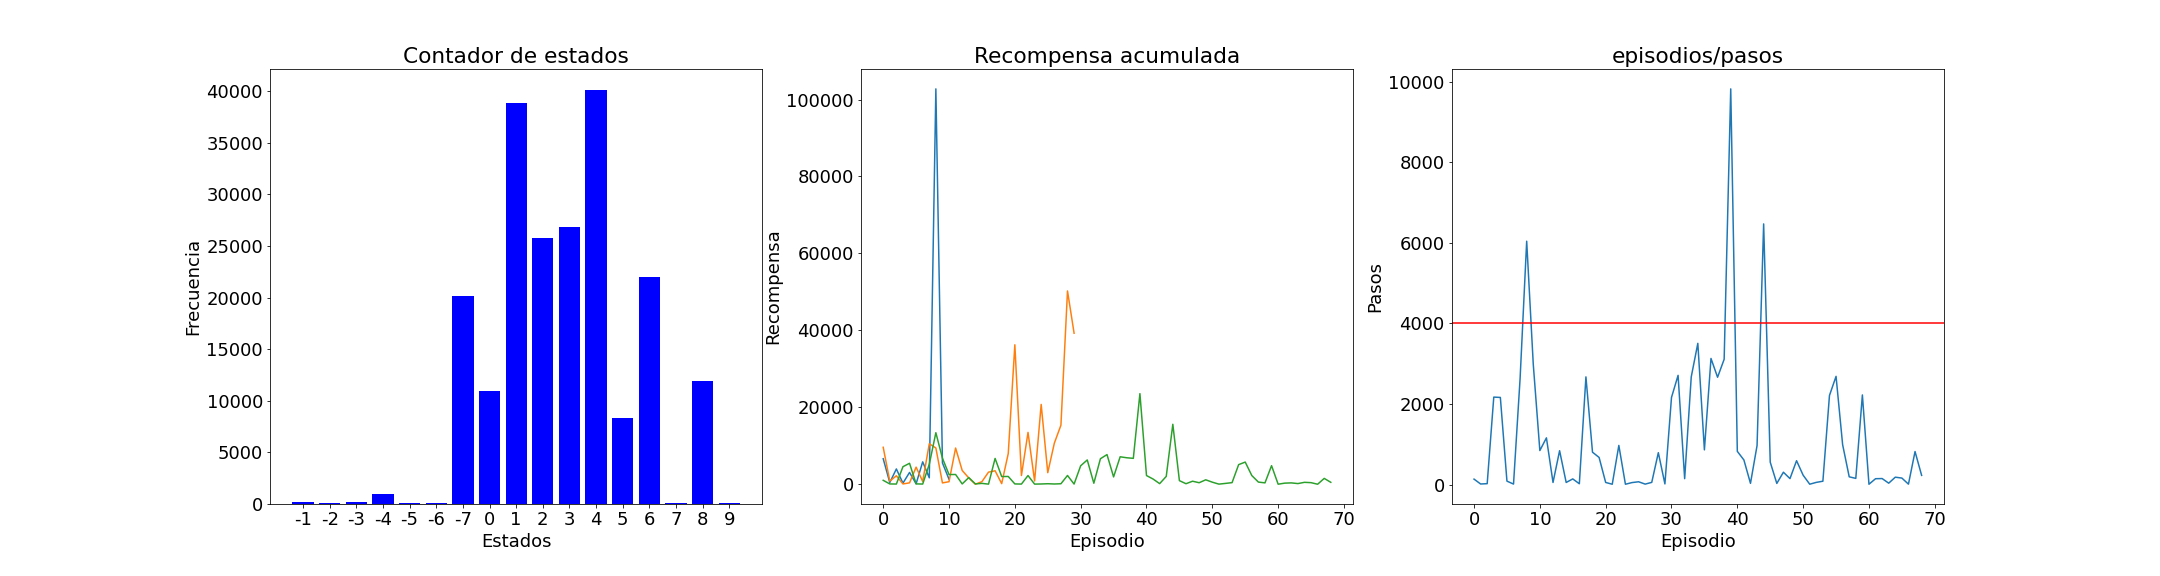
\includegraphics[width=1\columnwidth]{./figures/anexos/nurburgring_simple_1.png}
    \caption{Gráfica de resultados del entrenamiento en el Nürburgring con un conjunto de acciones simple y 1 punto de nivel de percepción.}
\end{figure}

\begin{table}[ht!]
\centering
\begin{tabular}{|
>{\columncolor[HTML]{EFEFEF}}l |c|c|c|}
\hline
\multicolumn{4}{|c|}{\cellcolor[HTML]{EFEFEF}\textbf{Tabla de entrenamiento en Nürburgring}}                                   \\ \hline
\textbf{Entrenamiento} & \cellcolor[HTML]{3685BB}\textbf{1} & \cellcolor[HTML]{FF8215}\textbf{2} & \cellcolor[HTML]{2CA02C}\textbf{3} \\ \hline
\textbf{Vuelta completada}         & Sí        & Sí        & Sí         \\ \hline
\textbf{Tiempo hasta completar}    & 07:43 min & 10:34 min & 11:57 min  \\ \hline
\textbf{Épocas hasta completar}    & 8         & 8         & 8         \\ \hline
\textbf{Valor de $\epsilon$ final} & 0.84      & 0.83      & 0.80       \\ \hline
\textbf{Tamaño de la Tabla-Q}      & 26        & 34        & 41         \\ \hline
\textbf{Nº total de épocas}        & 11        & 30        & 69        \\ \hline
\end{tabular}
\caption{Resultados del entrenamiento en el Nürburgring con un conjunto de acciones simple y 1 punto de nivel de percepción.}
\label{tab:simple_circuit-medium-1}
\end{table}



\newpage
%%%%%%%%%%%%%%%%%%%%%%%%%%%%%%%%%%%%%%%%%%%%%%%%%%%%%%%%%%%%%%%%%%%%%%%%%%%%%%%%%%%%%%%%%%%%%%%%%%%%%%%%%%%%%%%%%%%%
\subsection{Circuito de Nürburgring, conjunto de acciones medio y un punto de percepción}

\begin{figure}[!ht]
    \centering 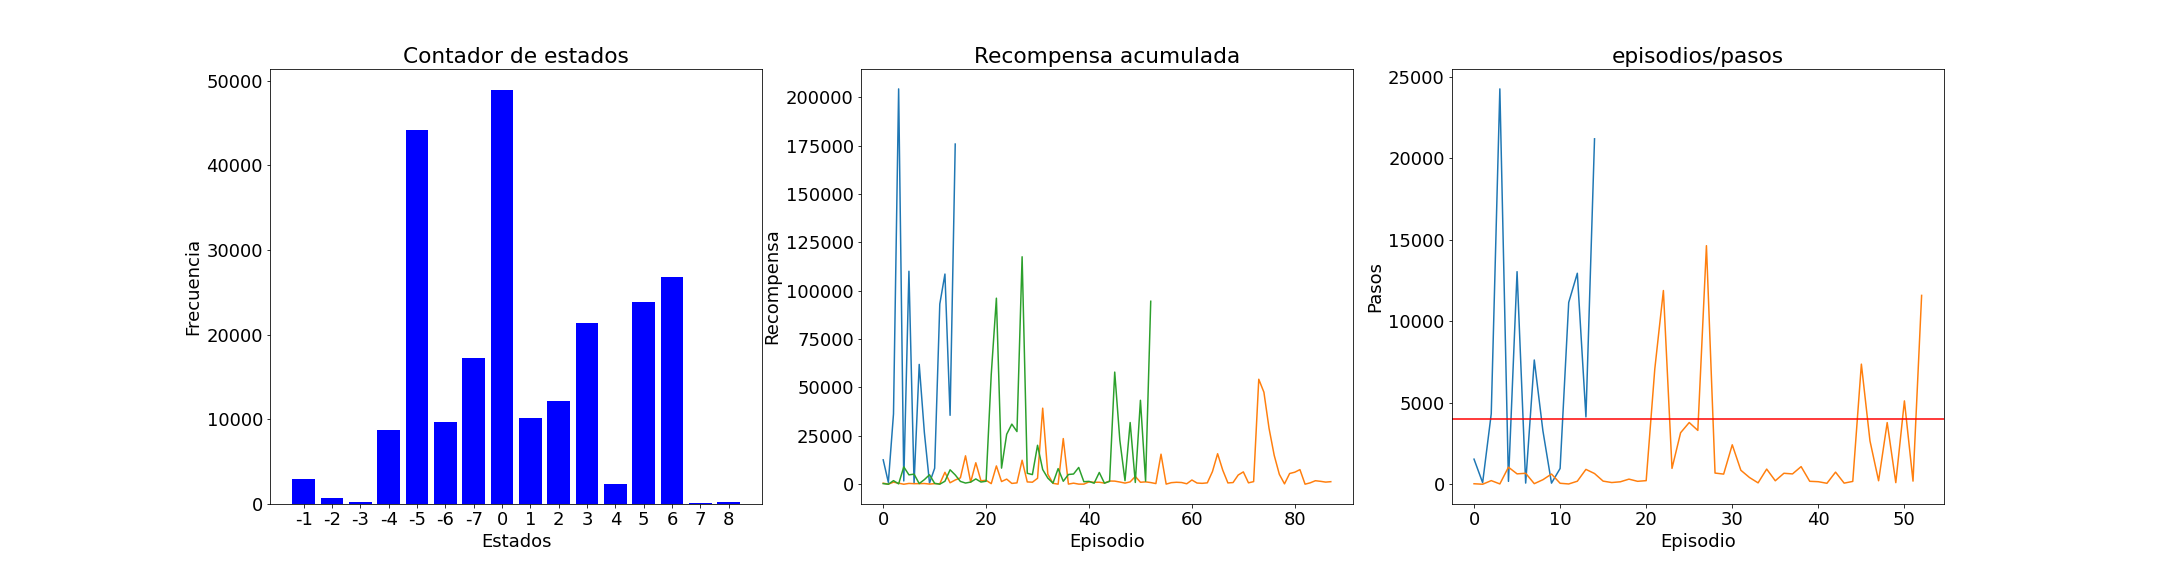
\includegraphics[width=1\columnwidth]{./figures/anexos/nurburgring_medium_1.png}
    \caption{Gráfica de resultados del entrenamiento en el Nürburgring con un conjunto de acciones medio y 1 punto de nivel de percepción.}
\end{figure}

\begin{table}[ht!]
\centering
\begin{tabular}{|
>{\columncolor[HTML]{EFEFEF}}l |c|c|c|}
\hline
\multicolumn{4}{|c|}{\cellcolor[HTML]{EFEFEF}\textbf{Tabla de entrenamiento en Nürburgring}}                                   \\ \hline
\textbf{Entrenamiento} & \cellcolor[HTML]{3685BB}\textbf{1} & \cellcolor[HTML]{FF8215}\textbf{2} & \cellcolor[HTML]{2CA02C}\textbf{3} \\ \hline
\textbf{Vuelta completada}         & Sí        & Sí        & Sí         \\ \hline
\textbf{Tiempo hasta completar}    & 10:34 min & 24:53 min & 11:25 min  \\ \hline
\textbf{Épocas hasta completar}    & 3         & 31         & 21         \\ \hline
\textbf{Recompensa en esa época}   & 18803     & 3646      & 7846         \\ \hline
\textbf{Valor de $\epsilon$ final} & 0.84      & 0.78      & 0.81       \\ \hline
\textbf{Tamaño de la Tabla-Q}      & 31        & 53        & 41         \\ \hline
\textbf{Nº total de épocas}        & 15        & 88        & 53        \\ \hline
\end{tabular}
\caption{Resultados del entrenamiento en el Nürburgring con un conjunto de acciones medio y 1 punto de nivel de percepción.}
\label{tab:simple_circuit-medium-1}
\end{table}

\newpage
%%%%%%%%%%%%%%%%%%%%%%%%%%%%%%%%%%%%%%%%%%%%%%%%%%%%%%%%%%%%%%%%%%%%%%%%%%%%%%%%%%%%%%%%%%%%%%%%%%%%%%%%%%%%%%%%%%%%
\subsection{Circuito de Nürburgring, conjunto de acciones difícil y un punto de percepción}

\begin{figure}[!ht]
    \centering 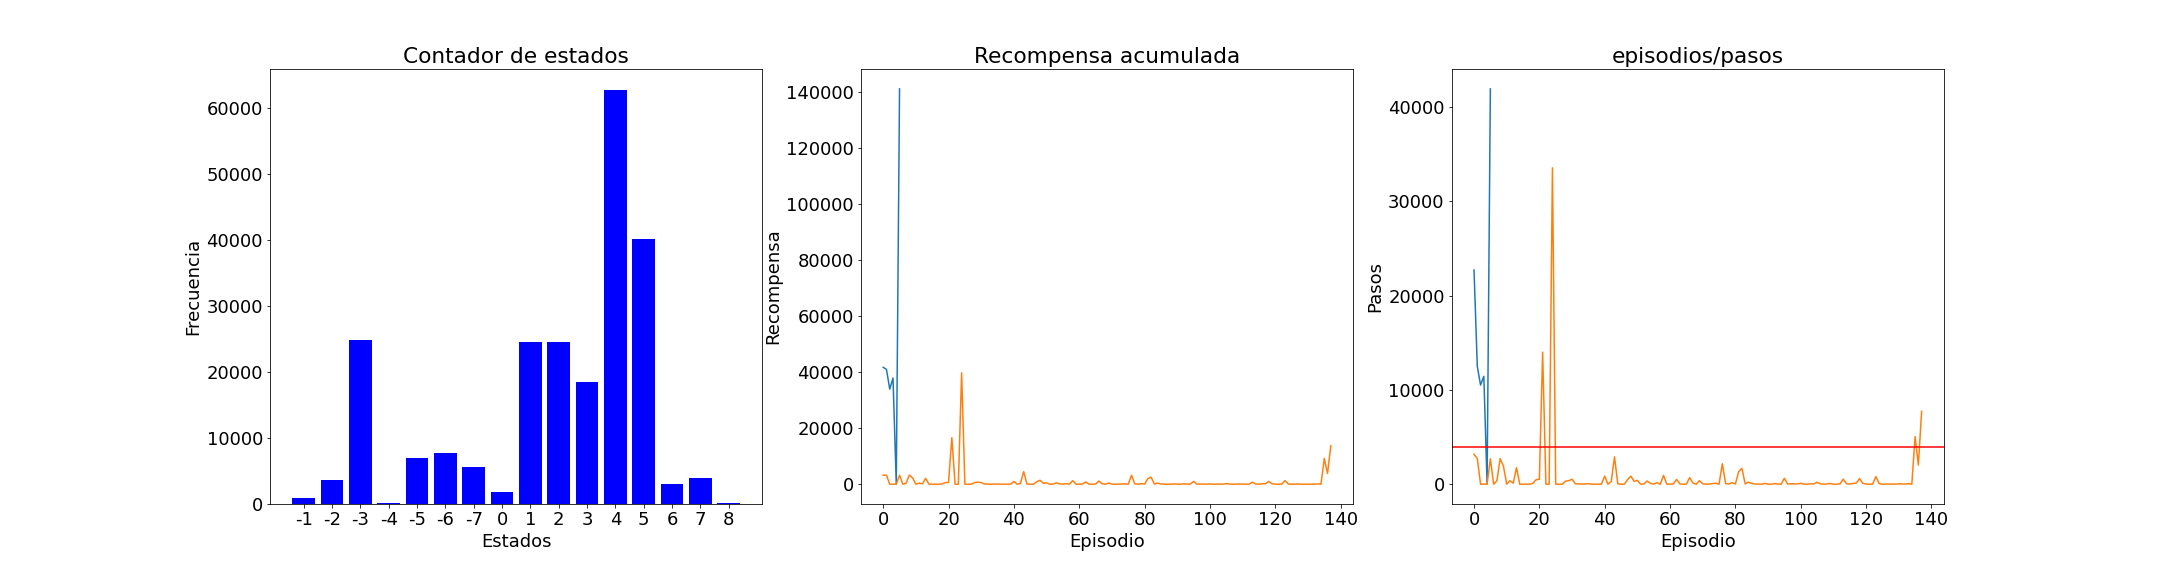
\includegraphics[width=1\columnwidth]{./figures/anexos/nurburgring_hard_1.png}
    \caption{Gráfica de resultados del entrenamiento en el Nürburgring con un conjunto de acciones difícil y 1 punto de nivel de percepción.}
\end{figure}

\begin{table}[ht!]
\centering
\begin{tabular}{|
>{\columncolor[HTML]{EFEFEF}}l |c|c|c|}
\hline
\multicolumn{4}{|c|}{\cellcolor[HTML]{EFEFEF}\textbf{Tabla de entrenamiento en Nürburgring}}                                   \\ \hline
\textbf{Entrenamiento} & \cellcolor[HTML]{3685BB}\textbf{1} & \cellcolor[HTML]{FF8215}\textbf{2} & \cellcolor[HTML]{2CA02C}\textbf{3} \\ \hline
\textbf{Vuelta completada}         & Sí        & Sí        & Sí         \\ \hline
\textbf{Tiempo hasta completar}    & 29:13 min & 22:47 min & 3:56 min  \\ \hline
\textbf{Épocas hasta completar}    & 2         & 21        & 1         \\ \hline
\textbf{Valor de $\epsilon$ final} & 0.85      & 0.72      & 0.85       \\ \hline
\textbf{Tamaño de la Tabla-Q}      & 27        & 71        & 10         \\ \hline
\textbf{Nº total de épocas}        & 6        & 138        & 1        \\ \hline
\end{tabular}
\caption{Resultados del entrenamiento en el Nürburgring con un conjunto de acciones difícil y 1 punto de nivel de percepción.}
\label{tab:simple_circuit-medium-1}
\end{table}












%%%%%%%%%%%%%%%%%%%%%%%%%%%%%%%%%%%%%%%%%%%%%%%%%%%%%%%%%%%%%%%%%%%%%%%%%%%%%%%%%%%%%%%%%%%%%%%%%%%%%%%%%%%%%%%%%%%%
\subsection{Circuito de Nürburgring, conjunto de acciones simple y dos puntos de percepción}


\begin{figure}[!ht]
    \centering 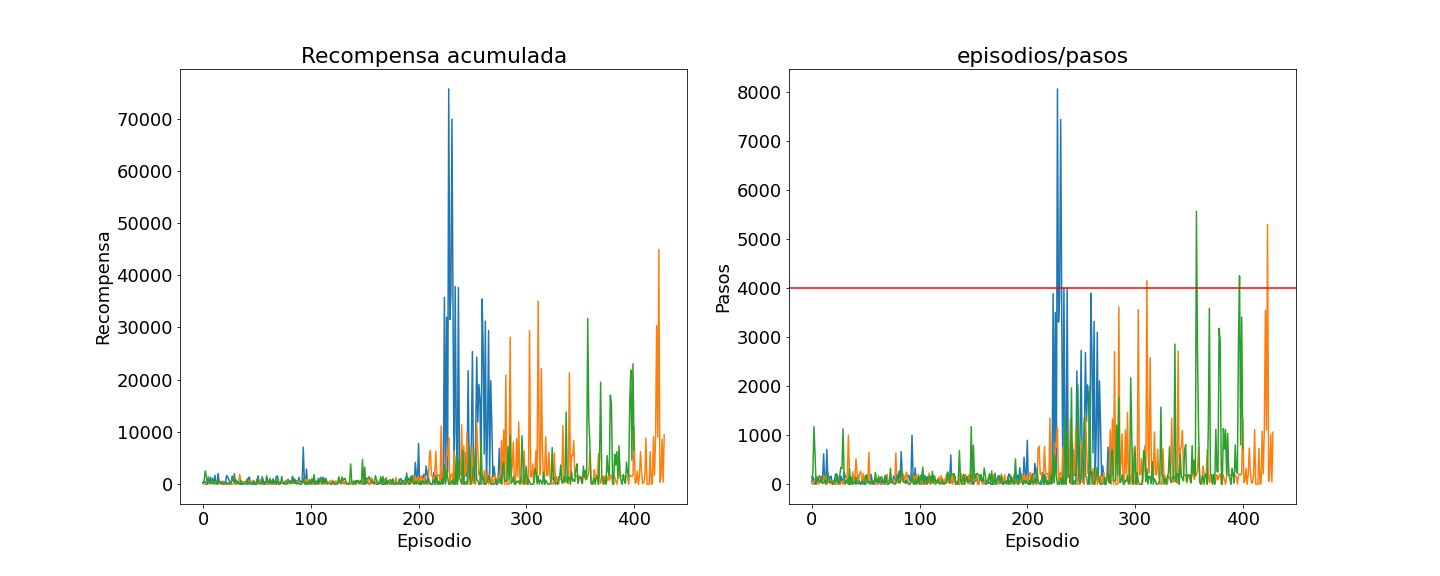
\includegraphics[width=1\columnwidth]{./figures/anexos/nurburgring_simple_2.png}
    \caption{Gráfica de resultados del entrenamiento en el Nürburgring con un conjunto de acciones simple y 2 puntos de nivel de percepción.}
\end{figure}

\begin{figure}[!ht]
    \centering 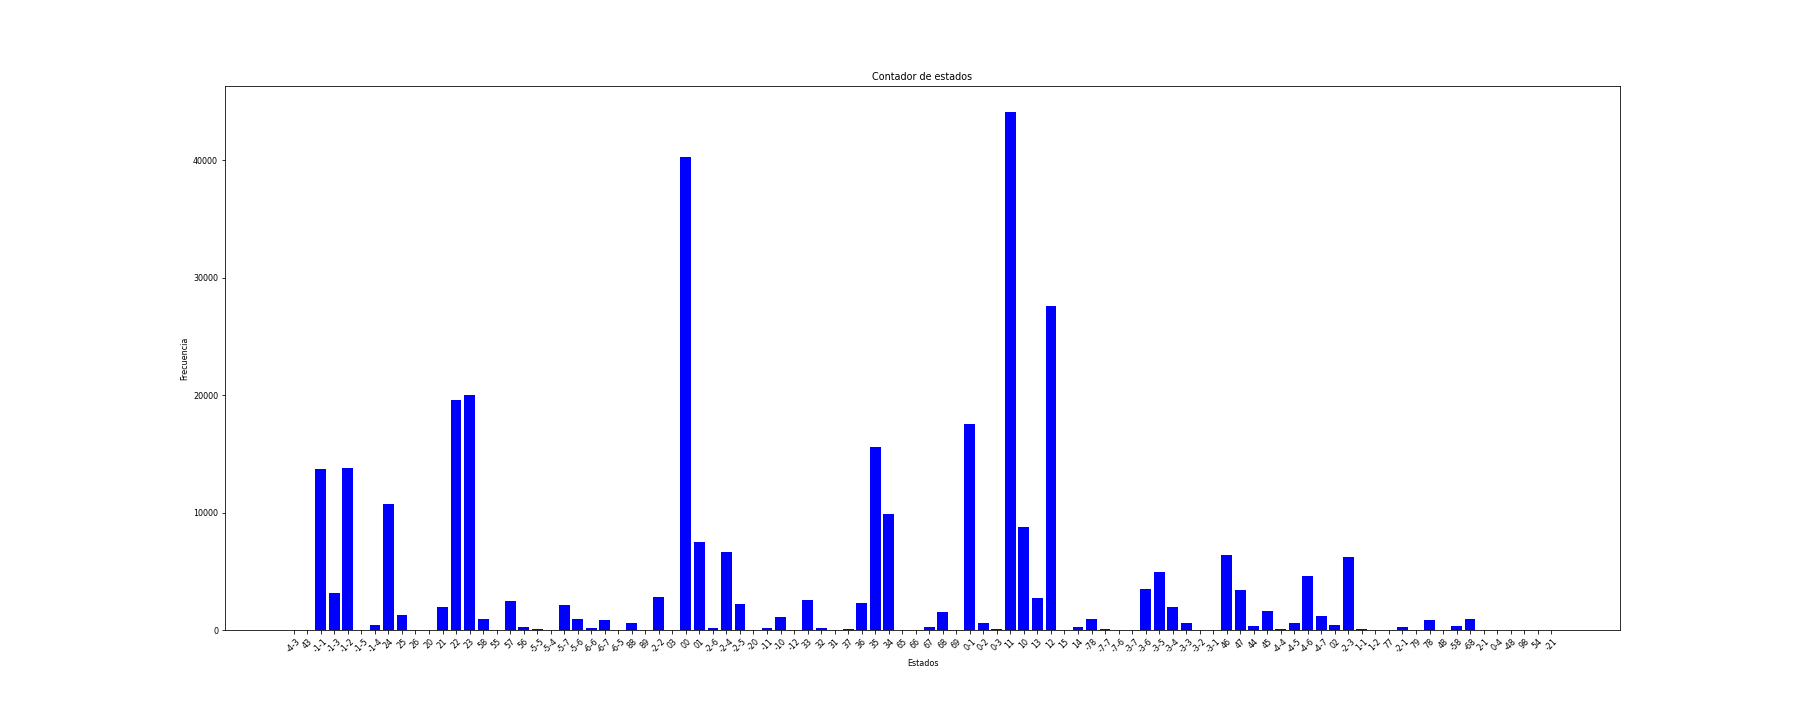
\includegraphics[width=1\columnwidth]{./figures/anexos/states_counter_nurburgring_simple_2.png}
    \caption{Gráfica de resultados de la distribución de los estados.}
\end{figure}


\begin{table}[ht!]
\centering
\begin{tabular}{|
>{\columncolor[HTML]{EFEFEF}}l |c|c|c|}
\hline
\multicolumn{4}{|c|}{\cellcolor[HTML]{EFEFEF}\textbf{Tabla de entrenamiento en Nürburgring}}                                   \\ \hline
\textbf{Entrenamiento} & \cellcolor[HTML]{3685BB}\textbf{1} & \cellcolor[HTML]{FF8215}\textbf{2} & \cellcolor[HTML]{2CA02C}\textbf{3} \\ \hline
\textbf{Vuelta completada}         & Sí        & Sí        & Sí         \\ \hline
\textbf{Tiempo hasta completar}    & 29:31 min & 52:30 min & 1:15:52 horas  \\ \hline
\textbf{Épocas hasta completar}    & 224         & 285        & 357         \\ \hline
\textbf{Valor de $\epsilon$ final} & 0.61      & 0.51      & 0.53       \\ \hline
\textbf{Tamaño de la Tabla-Q}      & 171        & 149        & 175         \\ \hline
\textbf{Nº total de épocas}        & 281        & 429        & 401        \\ \hline
\end{tabular}
\caption{Resultados del entrenamiento en el Nürburgring con un conjunto de acciones simple y 2 puntos de nivel de percepción.}
\label{tab:simple_circuit-medium-1}
\end{table}

\newpage
%%%%%%%%%%%%%%%%%%%%%%%%%%%%%%%%%%%%%%%%%%%%%%%%%%%%%%%%%%%%%%%%%%%%%%%%%%%%%%%%%%%%%%%%%%%%%%%%%%%%%%%%%%%%%%%%%%%%
\subsection{Circuito de Nürburgring, conjunto de acciones difícil y dos puntos de percepción}

\begin{figure}[!ht]
    \centering 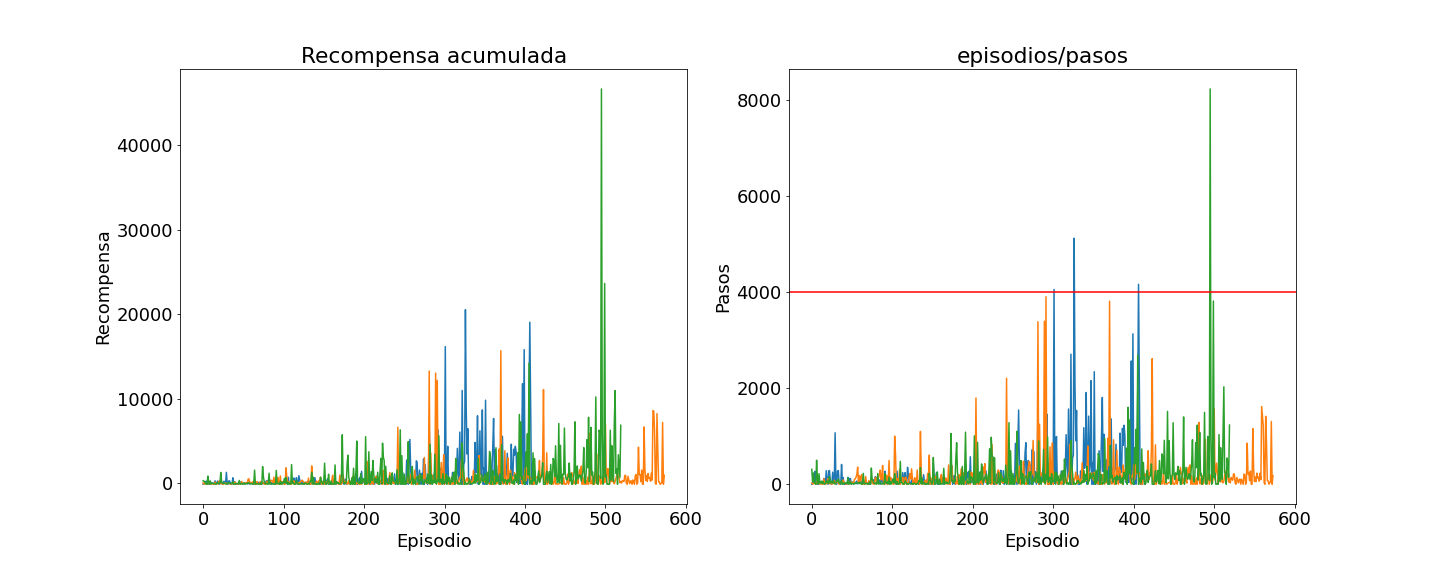
\includegraphics[width=1\columnwidth]{./figures/anexos/nurburgring_hard_2.png}
    \caption{Gráfica de resultados del entrenamiento en el Nürburgring con un conjunto de acciones difícil y 2 puntos de nivel de percepción.}
\end{figure}

\begin{figure}[!ht]
    \centering 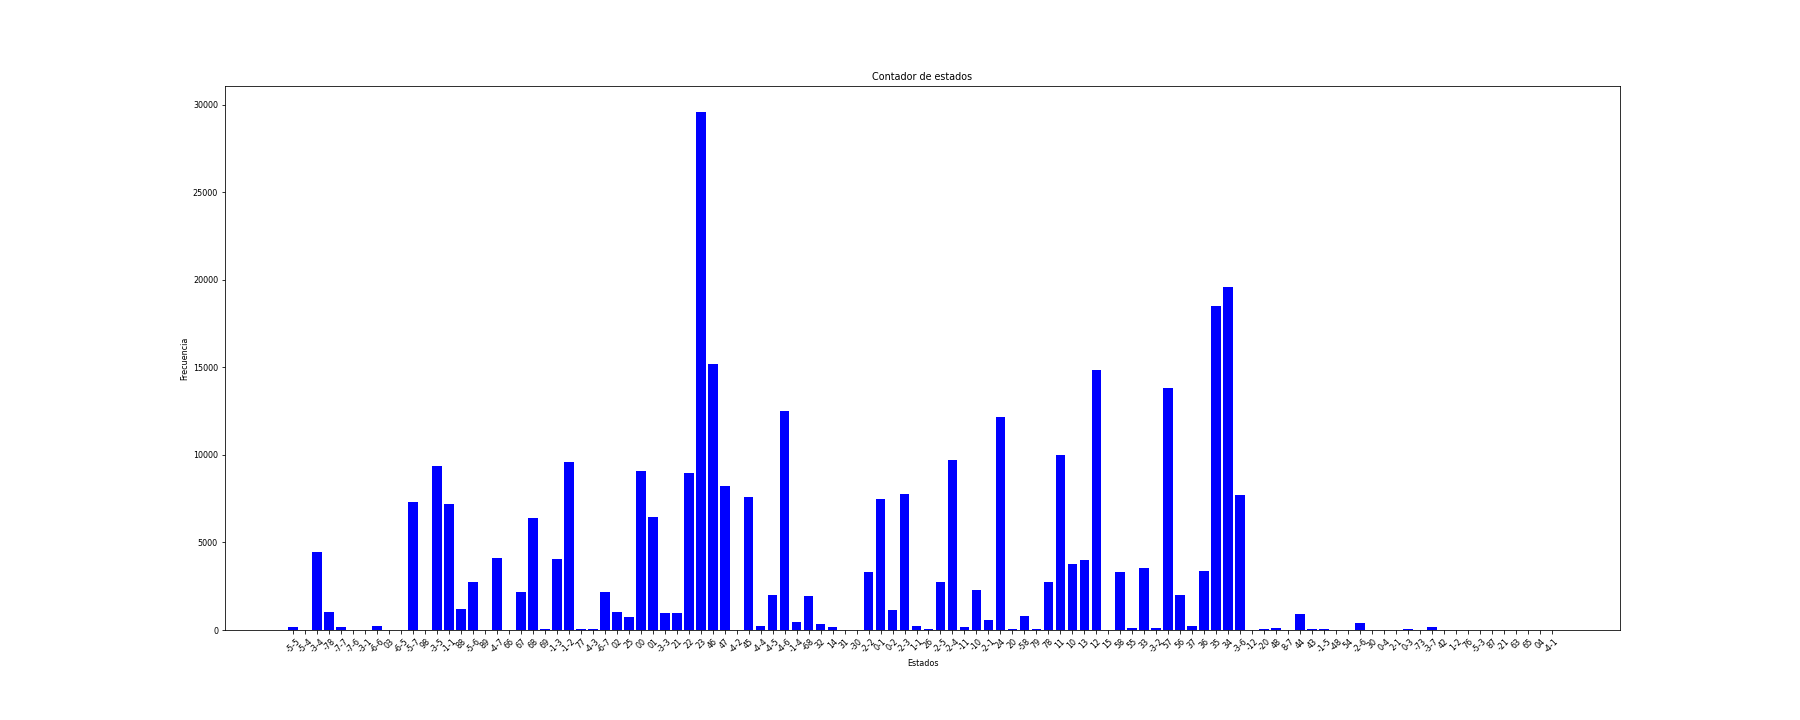
\includegraphics[width=1\columnwidth]{./figures/anexos/states_counter_nurburgring_hard_2.png}
    \caption{Gráfica de resultados de la distribución de los estados.}
\end{figure}


\begin{table}[ht!]
\centering
\begin{tabular}{|
>{\columncolor[HTML]{EFEFEF}}l |c|c|c|}
\hline
\multicolumn{4}{|c|}{\cellcolor[HTML]{EFEFEF}\textbf{Tabla de entrenamiento en Nürburgring}}                                   \\ \hline
\textbf{Entrenamiento} & \cellcolor[HTML]{3685BB}\textbf{1} & \cellcolor[HTML]{FF8215}\textbf{2} & \cellcolor[HTML]{2CA02C}\textbf{3} \\ \hline
\textbf{Vuelta completada}         & Sí        & Sí        & Sí         \\ \hline
\textbf{Tiempo hasta completar}    & 44:21 min & 50:59 min & 1:38 min  \\ \hline
\textbf{Épocas hasta completar}    & 301         & 291        & 495         \\ \hline
\textbf{Valor de $\epsilon$ final} & 0.52      & 0.43      & 0.45       \\ \hline
\textbf{Tamaño de la Tabla-Q}      & 239        & 248        & 262         \\ \hline
\textbf{Nº total de épocas}        & 415        & 574        & 528        \\ \hline
\end{tabular}
\caption{Resultados del entrenamiento en el Nürburgring con un conjunto de acciones difícil y 2 puntos de nivel de percepción.}
\label{tab:simple_circuit-medium-1}
\end{table}


\newpage
%%%%%%%%%%%%%%%%%%%%%%%%%%%%%%%%%%%%%%%%%%%%%%%%%%%%%%%%%%%%%%%%%%%%%%%%%%%%%%%%%%%%%%%%%%%%%%%%%%%%%%%%%%%%%%%%%%%%
\subsection{Circuito de Nürburgring, conjunto de acciones simple y tres puntos de percepción}

El estado más frecuente es el  $(0, -1, -4)$ con un valor de $16114$ veces.

\begin{figure}[!ht]
    \centering 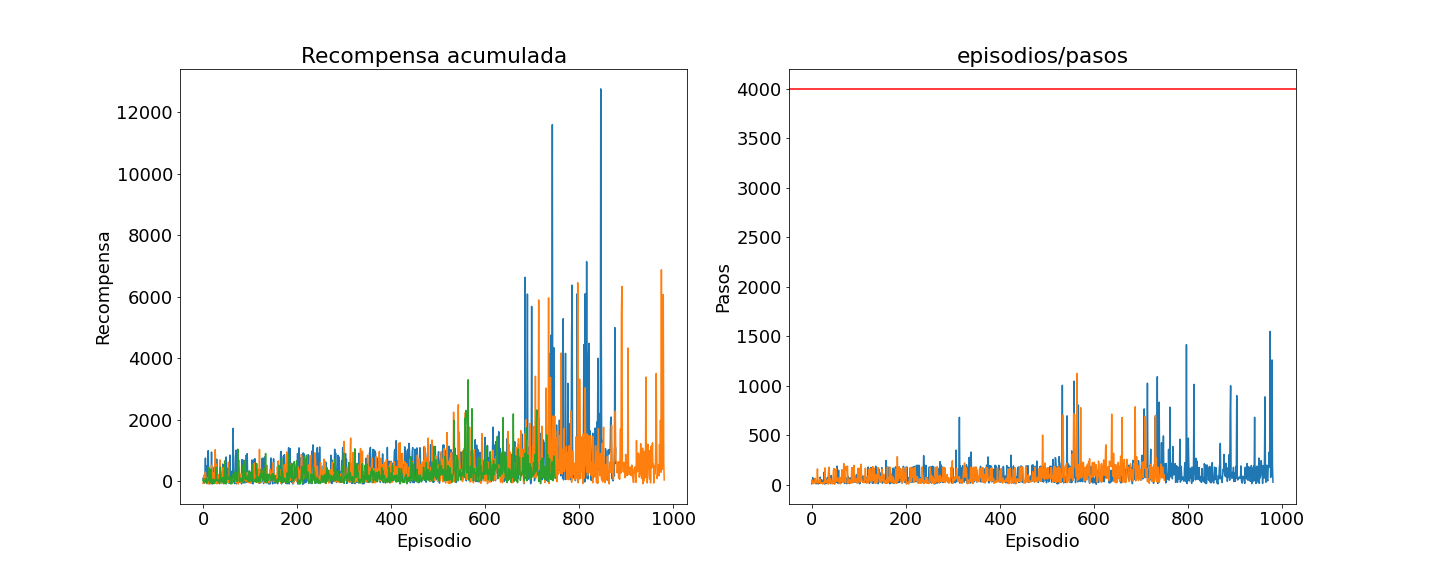
\includegraphics[width=1\columnwidth]{./figures/anexos/nurburgring_simple_3.png}
    \caption{Gráfica de resultados del entrenamiento en el Nürburgring con un conjunto de acciones fácil y 3 puntos de nivel de percepción.}
\end{figure}

\begin{figure}[!ht]
    \centering 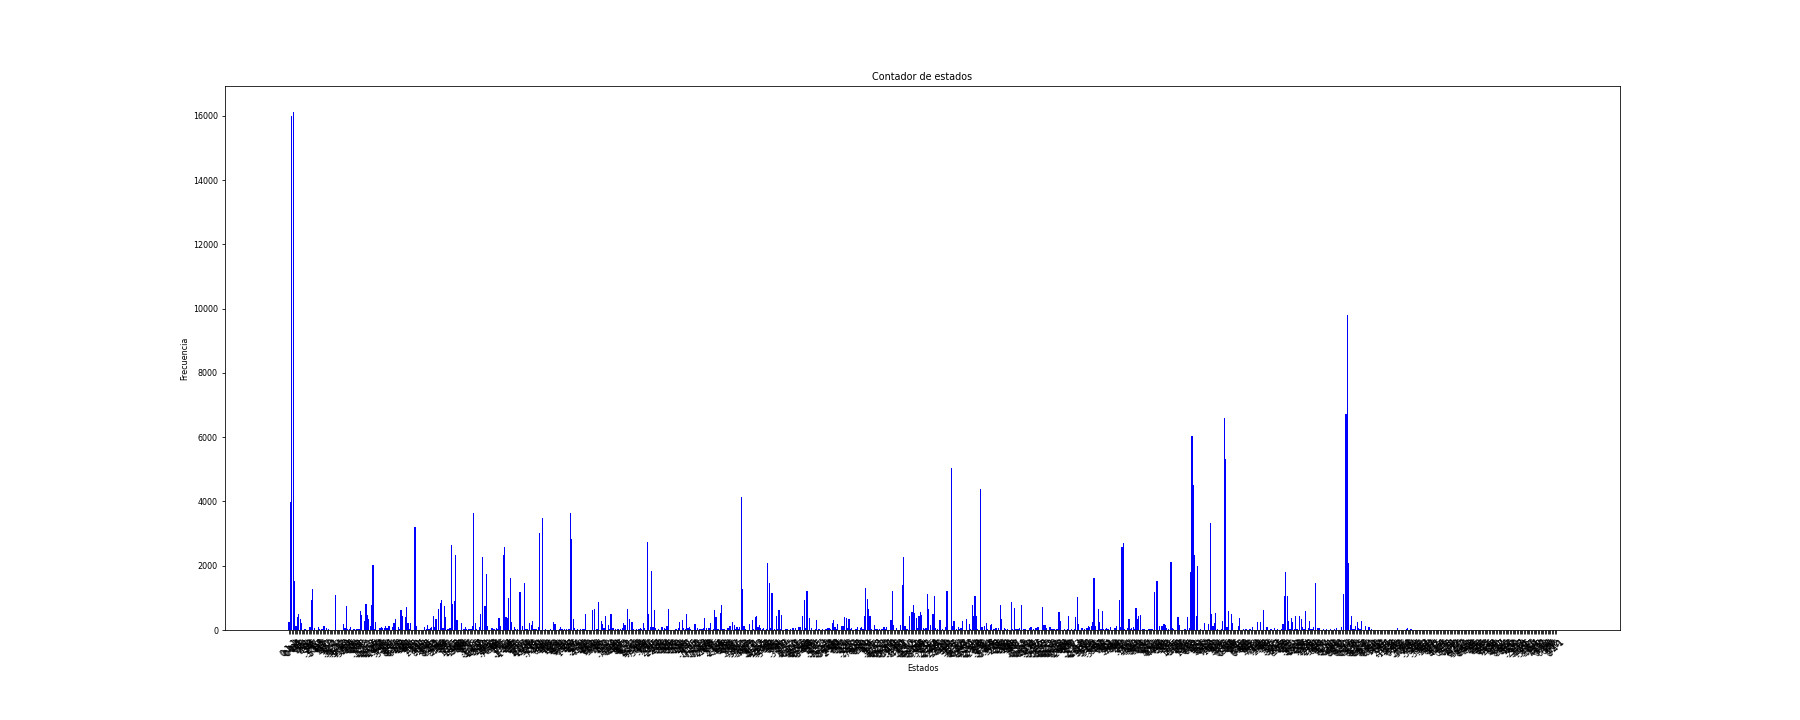
\includegraphics[width=1\columnwidth]{./figures/anexos/states_counter_nurburgring_simple_3.png}
    \caption{Gráfica de resultados de la distribución de los estados.}
\end{figure}

\begin{table}[ht!]
\centering
\begin{tabular}{|
>{\columncolor[HTML]{EFEFEF}}l |c|c|c|}
\hline
\multicolumn{4}{|c|}{\cellcolor[HTML]{EFEFEF}\textbf{Tabla de entrenamiento en el Nürburgring}}                                   \\ \hline
\textbf{Entrenamiento} & \cellcolor[HTML]{3685BB}\textbf{1} & \cellcolor[HTML]{FF8215}\textbf{2} & \cellcolor[HTML]{2CA02C}\textbf{3} \\ \hline
\textbf{Vuelta completada}         & No        & No          & No        \\ \hline
\textbf{Tiempo hasta completar}    & $\infty$  & $\infty$    & $\infty$ \\ \hline
\textbf{Épocas hasta completar}    & -         & -      & -              \\ \hline
\textbf{Valor de $\epsilon$ final} & 0.28      & 0.25        & 0.29      \\ \hline
\textbf{Tamaño de la Tabla-Q}      & 1199       & 1194         & 1191        \\ \hline
\textbf{Nº total de épocas}        & 911       & 892         & 771        \\ \hline
\end{tabular}
\caption{Resultados del entrenamiento en el Nürburgring con un conjunto de acciones simple y 3 puntos de nivel de percepción.}
\label{tab:simple_circuit-medium-1}
\end{table}

\newpage
%%%%%%%%%%%%%%%%%%%%%%%%%%%%%%%%%%%%%%%%%%%%%%%%%%%%%%%%%%%%%%%%%%%%%%%%%%%%%%%%%%%%%%%%%%%%%%%%%%%%%%%%%%%%%%%%%%%%
\subsection{Circuito de Nürburgring, conjunto de acciones medio y tres puntos de percepción}

El estado más frecuente es el  $(1,3,6)$ con un valor de $9161$ veces.

\begin{figure}[!ht]
    \centering 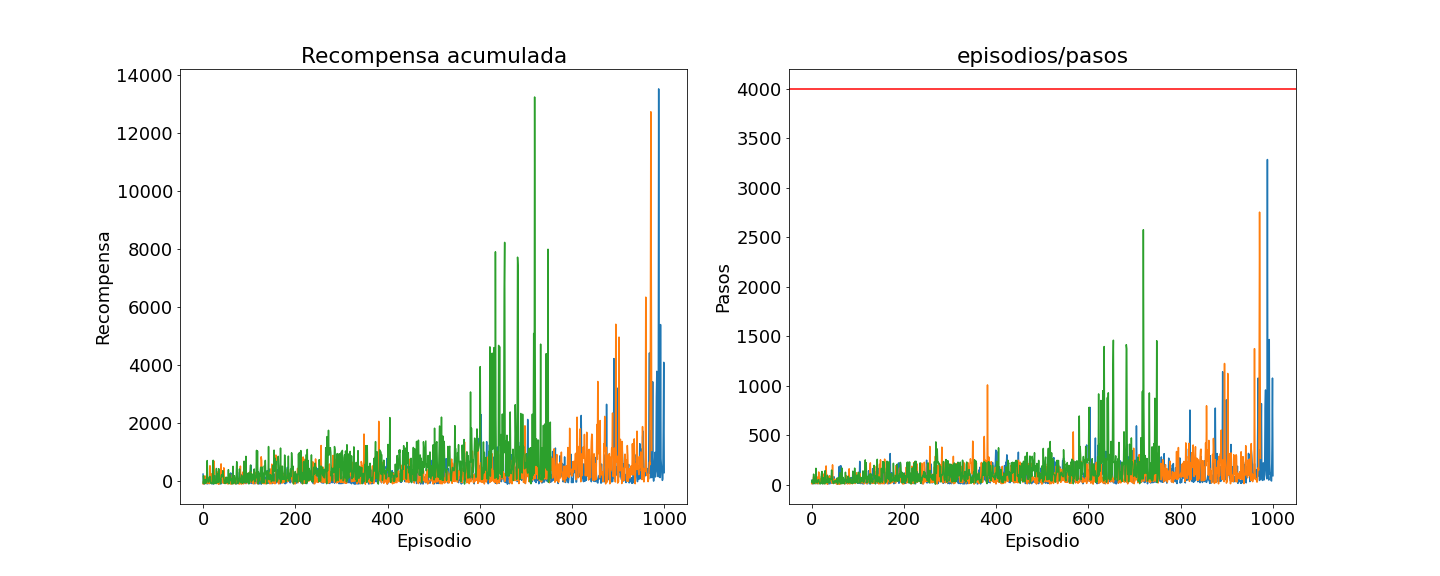
\includegraphics[width=1\columnwidth]{./figures/anexos/nurburgring_medium_3.png}
    \caption{Gráfica de resultados del entrenamiento en el Nürburgring con un conjunto de acciones medio y 3 puntos de nivel de percepción.}
\end{figure}

\begin{figure}[!ht]
    \centering 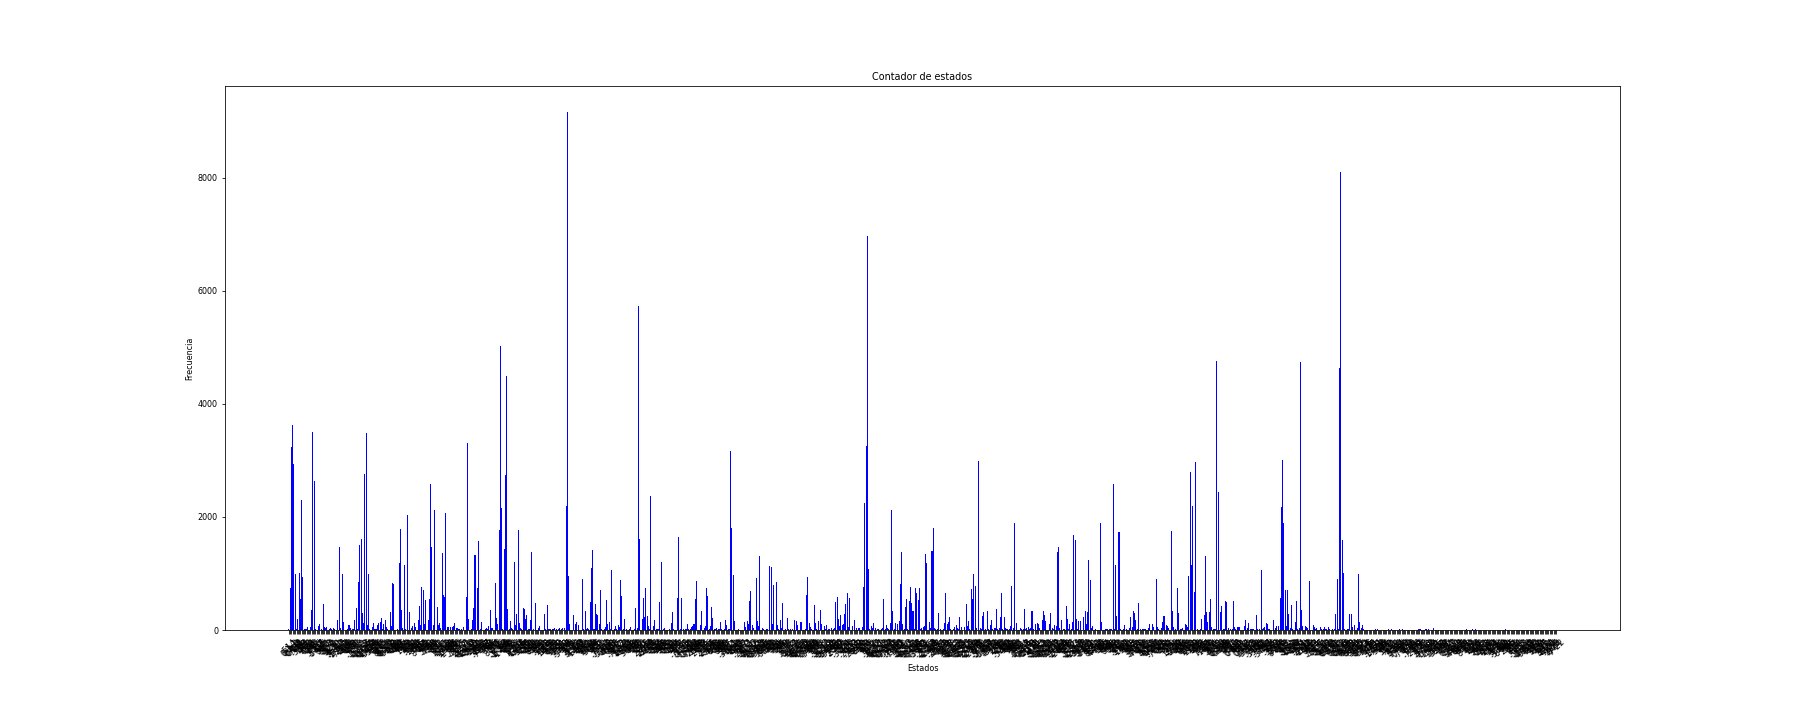
\includegraphics[width=1\columnwidth]{./figures/anexos/states_counter_nurburgring_medium_3.png}
    \caption{Gráfica de resultados de la distribución de los estados.}
\end{figure}

\begin{table}[ht!]
\centering
\begin{tabular}{|
>{\columncolor[HTML]{EFEFEF}}l |c|c|c|}
\hline
\multicolumn{4}{|c|}{\cellcolor[HTML]{EFEFEF}\textbf{Tabla de entrenamiento en el Nürburgring}}                                   \\ \hline
\textbf{Entrenamiento} & \cellcolor[HTML]{3685BB}\textbf{1} & \cellcolor[HTML]{FF8215}\textbf{2} & \cellcolor[HTML]{2CA02C}\textbf{3} \\ \hline
\textbf{Vuelta completada}         & No        & No          & No        \\ \hline
\textbf{Tiempo hasta completar}    & $\infty$  & $\infty$    & $\infty$ \\ \hline
\textbf{Épocas hasta completar}    & -         & -      & -              \\ \hline
\textbf{Valor de $\epsilon$ final} & 0.24      & 0.25        & 0.34      \\ \hline
\textbf{Tamaño de la Tabla-Q}      & 1003       & 976         & 755        \\ \hline
\textbf{Nº total de épocas}        & 303       & 1824         & 1064        \\ \hline
\end{tabular}
\caption{Resultados del entrenamiento en el Nürburgring con un conjunto de acciones medio y 3 puntos de nivel de percepción.}
\label{tab:simple_circuit-medium-1}
\end{table}

\newpage
%%%%%%%%%%%%%%%%%%%%%%%%%%%%%%%%%%%%%%%%%%%%%%%%%%%%%%%%%%%%%%%%%%%%%%%%%%%%%%%%%%%%%%%%%%%%%%%%%%%%%%%%%%%%%%%%%%%%
\subsection{Circuito de Nürburgring, conjunto de acciones difícil y tres puntos de percepción}

El estado más frecuente es el  $(2,4,7)$ con un valor de $8707$ veces.

\begin{figure}[!ht]
    \centering 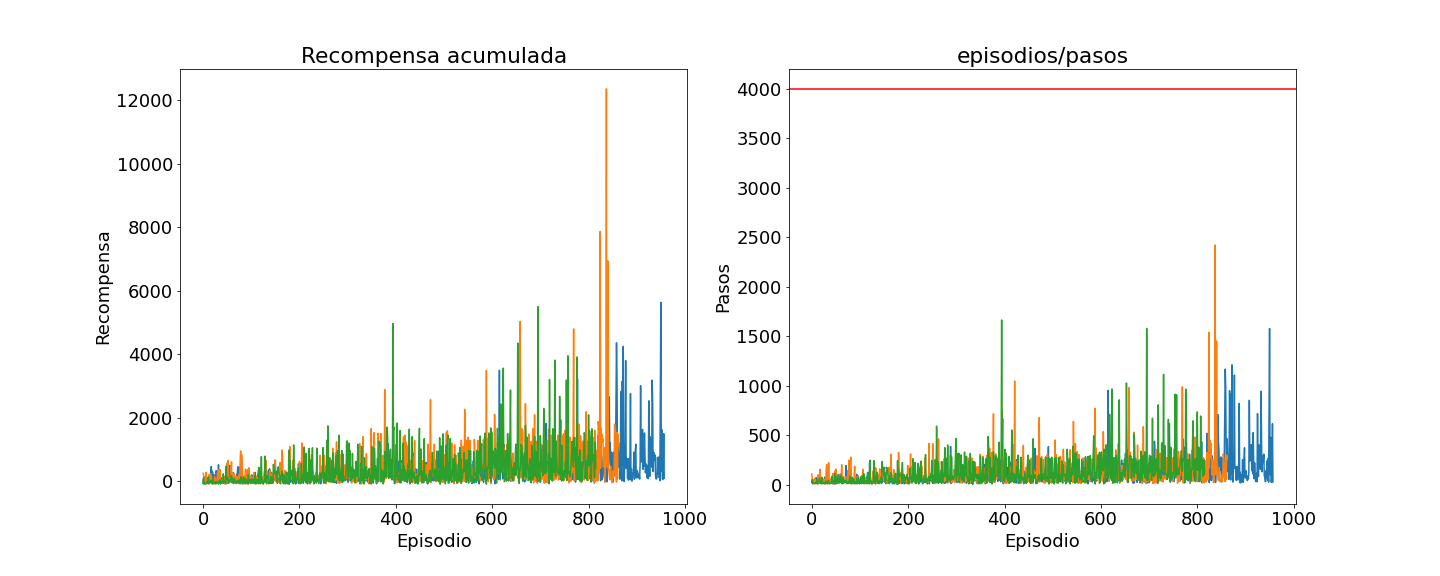
\includegraphics[width=1\columnwidth]{./figures/anexos/nurburgring_hard_3.png}
    \caption{Gráfica de resultados del entrenamiento en el Nürburgring con un conjunto de acciones difícil y 3 puntos de nivel de percepción.}
\end{figure}

\begin{figure}[!ht]
    \centering 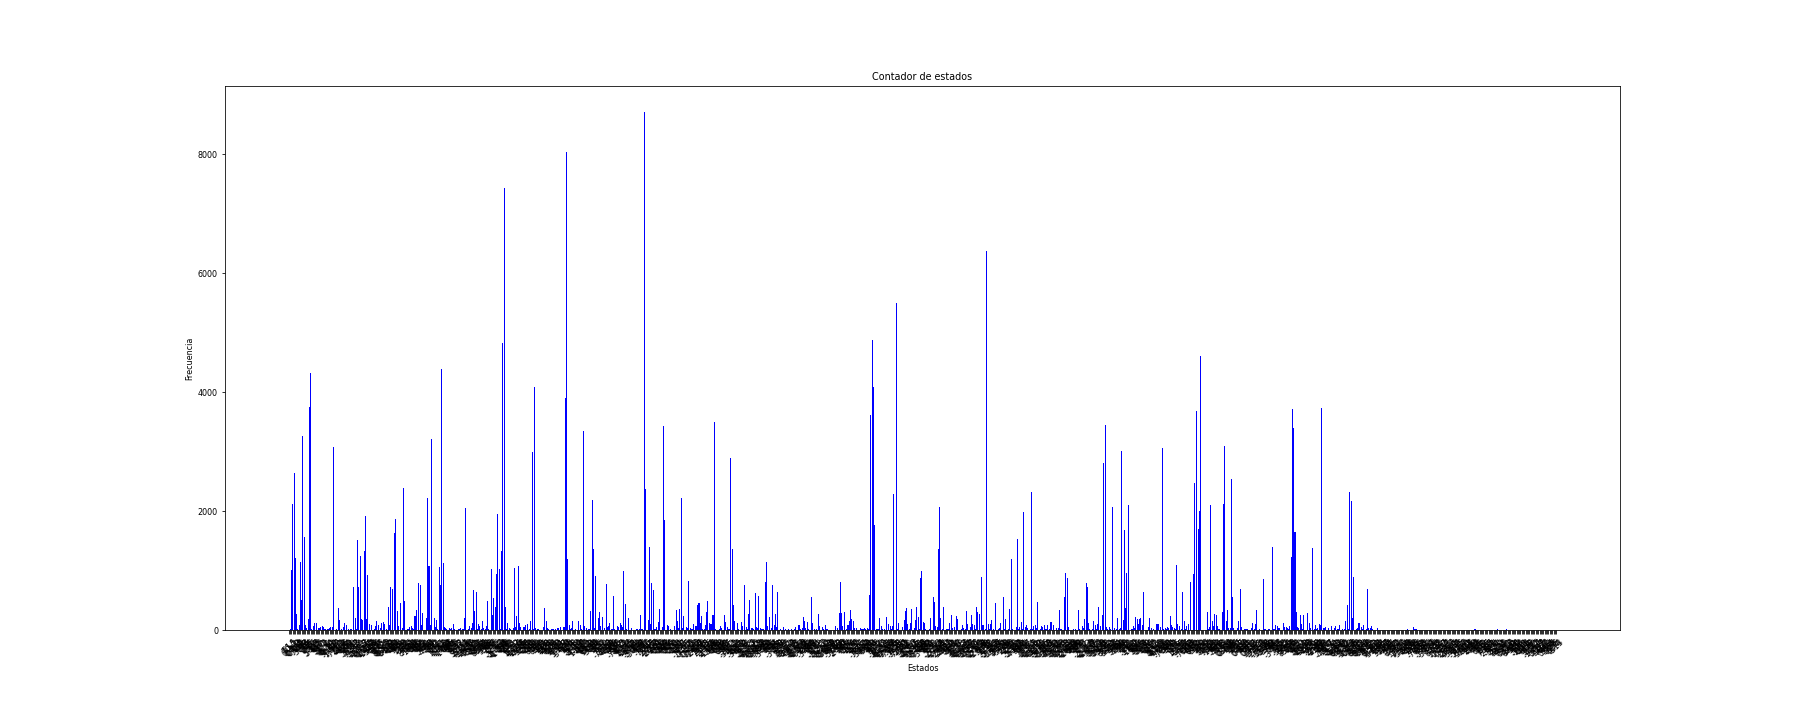
\includegraphics[width=1\columnwidth]{./figures/anexos/states_counter_nurburgring_hard_3.png}
    \caption{Gráfica de resultados de la distribución de los estados.}
\end{figure}

\begin{table}[ht!]
\centering
\begin{tabular}{|
>{\columncolor[HTML]{EFEFEF}}l |c|c|c|}
\hline
\multicolumn{4}{|c|}{\cellcolor[HTML]{EFEFEF}\textbf{Tabla de entrenamiento en el Nürburgring}}                                   \\ \hline
\textbf{Entrenamiento} & \cellcolor[HTML]{3685BB}\textbf{1} & \cellcolor[HTML]{FF8215}\textbf{2} & \cellcolor[HTML]{2CA02C}\textbf{3} \\ \hline
\textbf{Vuelta completada}         & No        & No          & No        \\ \hline
\textbf{Tiempo hasta completar}    & $\infty$  & $\infty$    & $\infty$ \\ \hline
\textbf{Épocas hasta completar}    & -         & -      & -              \\ \hline
\textbf{Valor de $\epsilon$ final} & 0.26      & 0.29        & 0.31      \\ \hline
\textbf{Tamaño de la Tabla-Q}      & 1577       & 1506         & 1466        \\ \hline
\textbf{Nº total de épocas}        & 958       & 863         & 816        \\ \hline
\end{tabular}
\caption{Resultados del entrenamiento en el Nürburgring con un conjunto de acciones difícil y 3 puntos de nivel de percepción.}
\label{tab:simple_circuit-medium-1}
\end{table}